\chapter{\label{ch:michel}Study of Michel Electrons in \protodune{}} 

%%%%%%%%%%%%%%%%%%%%%%%%%%%%%%%%%%%%%%%%%%%%%%%%%%%%%%%%%%%%%%%%%%%%%%%%%%%%%%%%
% FROM COS
%
% This chapter will cover the primary analysis of this thesis; a study of Michel
% electrons in the ProtoDUNE--SP detector which aims to investigate the agreement
% between data and simulation, and to provide an estimate of the energy scale
% uncertainty and energy scale bias for electrons in the 0--60 MeV range. 
% 
% The work done for this section is ongoing; preliminary work on this topic was
% presented in the report submitted for transfer of status. The rest of the work
% for this section is expected to be completed by the end of October 2019.
% 
% \noindent The work done as of writing for this chapter is as follows:
% \begin{itemize}[noitemsep,nolistsep]
% 	\item Event selection algorithm developed based on clustering of the Michel
% 	like hits discussed in the previous chapter.
% 	\begin{itemize}[noitemsep,nolistsep]
% 		\item Purity of > 98\% and efficiency of 5\% measured in ProtoDUNE--SP 
% 		simulations.
% 	\end{itemize}
% 	\item Two possible energy reconstruction algorithms developed.
% 	\begin{itemize}[noitemsep,nolistsep]
% 		\item Cone algorithm.
% 		\item Semantic segmentation algorithm with U-ResNet CNN architecture.
% 	\end{itemize}
% \end{itemize}
% 
% \noindent The work left to do is as follows:
% \begin{itemize}[noitemsep, nolistsep]
% 	\item Validation of algorithms on the real ProtoDUNE--SP data.
% 	\item Data MC comparison for Michel electron energy spectrum.
% 	\item Energy scale uncertainty and energy scale bias measurements with 
% 	measured Michel electron energy spectrum.
% \end{itemize}
% 
% \noindent An example Michel electron candidate event from the real ProtoDUNE--SP 
% data is given in figure \ref{fig:michel_event}.
% 
% \begin{figure}[h]
% 	\centering
% 	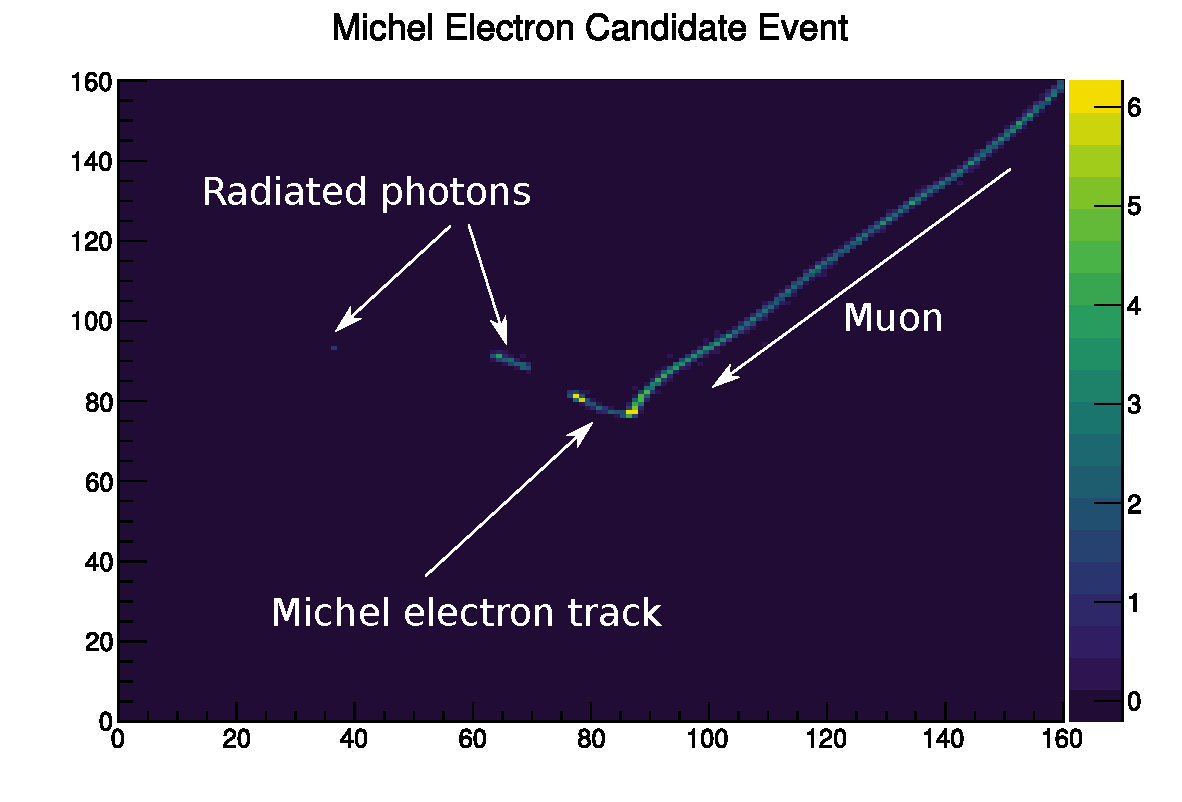
\includegraphics[width=0.7\textwidth]{figures/michel_candidate.pdf}
% 	\caption[Michel electron candidate event from ProtoDUNE--SP data.]{Michel 
% 	electron candidate event from ProtoDUNE--SP data.}
% 	\label{fig:michel_event}
% \end{figure}
%
%%%%%%%%%%%%%%%%%%%%%%%%%%%%%%%%%%%%%%%%%%%%%%%%%%%%%%%%%%%%%%%%%%%%%%%%%%%%%%%%

%%%%%%%%%%%%%%%%%%%%%%%%%%%%%%%%%%%%%%%%%%%%%%%%%%%%%%%%%%%%%%%%%%%%%%%%%%%%%%%%
% TODO: temporarily removed
% \subsubsection{Michel Electron Energy Reconstruction} \label{sec:michel_energy}
% TODO: decide if I want this.

% The true Michel electron energy includes contributions from scintillation light
% as well as radiated ionisation energy, which is not contained within the images
% used in reconstruction. In the noisy surface level environment of the
% \protodune{} TPC, it is not possible to reconstruct the scintillation light as
% part of the Michel electron events. Therefore, to estimate the total Michel 
% electron energy the reconstructed ionisation energy needs to be scaled to 
% account for these losses. As shown in Figure \ref{fig:michel_track_only},
% there is a none--linear correlation between the true Michel electron energy 
% and the available ionisation energy in reconstruction. Therefore, a quadratic 
% energy scaling factor was used to convert the reconstructed ionisation energy 
% into a reconstructed Michel electron energy. 
% 
% The energy scaling factor was estimated by fitting the reconstructed ionisation
% energy as a function of true Michel electron energy, with a quadratic 
% correction as shown in Figure \ref{fig:quadratic_fit}. This quadratic is then 
% inverted to give the reconstructed Michel electron energy,
% \begin{equation}
% 	E_{michel} = \left( \frac{E_{ion}}{a} - d \right)^{\frac{1}{2}} - \frac{b}{2a},
% 	\quad d = \frac{c}{a} - \left( \frac{b}{2a} \right)^2 
% \end{equation}
% where $E_{michel}$ is the reconstructed Michel electron energy, $E_{ion}$ is the
% reconstructed ionisation energy, and a, b, and c are the parameters from the
% quadratic fit. The fit gives,
% \begin{equation}
% 	a = TODO, \quad b = TODO, \quad c = TODO.
% \end{equation}
% \begin{figure}
% 	\centering
% 	% TODO
% 	
\includegraphics[width=\textwidth]{figures/placeholder.png}
% 	\caption
% 	[Quadratic fit of reconstructed ionisation energy vs true Michel electron
% 	enegry.]
% 	{Quadratic fit of reconstructed ionisation energy vs true Michel electron
% 	energy, which is used to calculate a quadratic energy correction factor.}
% 	\label{fig:quadratic_fit}
% \end{figure}
% 
% The reconstructed Michel electron energy spectrum is shown in Figure
% \ref{fig:reco_v_mich}. \mccorrect{TODO.}
% \begin{figure}
% 	\centering
% 	
\includegraphics[width=\textwidth]{figures/placeholder.png}
% 	\caption
% 	[Reconstructed Energy vs True Michel Electron Energy.]
% 	{Reconstructed Energy vs True Michel Electron Energy.}
% 	\label{fig:reco_v_mich}
% \end{figure}
% 
% The energy uncertainty and bias are estimated by fitting the fractional energy 
% difference between the reconstructed and true Michel electron energies as a 
% function of true Michel electron energy. The fractional energy difference, 
% defined as 
% \begin{equation}
% 	\Delta = \frac{E_{reco} - E_{true}}{E_{true}},
% \end{equation}
% is considered in bins of true Michel electron energy which are plotted in Figure
% \ref{fig:frac_diff_energy}. This difference is fit with a gaussian 
% distribution in each bin in order to estimate the energy uncertainty and bias 
% as a function of the true Michel electron energy.
% \begin{figure}
% 	\centering
% 	% TODO: make set of fits as a function of energy
% 	
\includegraphics[width=\textwidth]{figures/placeholder.png}
% 	\caption
% 	[Fractional energy difference between reconstructed and true Michel electron
% 	energy.]
% 	{Fractional energy difference between reconstructed and true Michel electron
% 	energy.}
% 	\label{fig:frac_diff_energy}
% \end{figure}
% 
% The energy resolution and bias as a function of true Michel electron energy are 
% estimated as the standard deviation and mean of the gaussian fit to the
% fractional energy difference in each energy bin, these values are plotted in
% Figure \ref{fig:res_and_bias_energy}. \mccorrect{TODO: analysis of results}.
% \begin{figure}
% 	\centering
% 	% TODO: make set of fits as a function of energy
% 	
\includegraphics[width=\textwidth]{figures/placeholder.png}
% 	\caption
% 	[Energy resolution and bias as a function of true Michel electron energy.]
% 	{Energy resolution and bias as a function of true Michel electron energy.}
% 	\label{fig:res_and_bias_energy}
% \end{figure}
%%%%%%%%%%%%%%%%%%%%%%%%%%%%%%%%%%%%%%%%%%%%%%%%%%%%%%%%%%%%%%%%%%%%%%%%%%%%%%%%

\minitoc

\noindent
Studying electrons in the tens of MeV energy range can provide valuable input 
into reconstruction techniques and energy uncertainty for the measurement of
astrophysical neutrinos from supernova bursts. Understanding the response of
LArTPC detectors to electrons in this range will be important for any large
scale LArTPC experiment wishing to study supernova bursts. At these energies
electron interactions have large contributions from both ionisation energy loss
and radiative energy loss and therefore they have a unique signature which is 
neither track--like or shower--like. Low--energy electrons therefore require 
unique reconstruction algorithms, to maximise the overall reconstruction 
performance. 

This chapter will discuss an approach to low--energy electron reconstruction 
in LArTPC detectors based on the use of convolutional neural networks and 
semantic segmentation. Michel electron events from \protodune{} will be used 
to test the performance of this technique and to provide an estimate of the 
energy uncertainty of LArTPC detectors for low--energy electrons.

In this chapter Section \ref{ME_LAr} will discuss the signature left by Michel
electrons in liquid argon, and the implications of this signature on
reconstructing Michel electron events in \protodune{}. This will be followed by
a discussion of the algorithm used to select Michel electron events in Section
\ref{ME_ES}. The Michel electron event reconstruction will be discussed in
Sections \ref{ME_R}. Finally, the results of this chapter and the implications
for the DUNE far detector will be summarised in Section \ref{ME_EU}.

\section{Michel Electrons in Liquid Argon} \label{ME_LAr}
Michel electrons are produced when a muon decays at rest. In vacuum, this 
decay gives rise to a characteristic energy spectrum which has a sharp 
cut--off at around 50 MeV, corresponding to half the muon mass. In matter it 
is also possible for $\mu^-$ to be captured on nuclei before they decay, this 
causes a broadening of the Michel electron spectrum for these events. A 
comparison of the Michel electron energy spectrum for free $\mu^+$ and 
captured $\mu^-$ is given in Figure \ref{fig:michel_spec}. The capture process 
occurs roughly 70\% of the time for negative muons in liquid argon, therefore, 
in \protodune{} the observed Michel electron energy spectrum is a combination 
of the two processes in roughly equal quantities.
\begin{figure}

	\centering
	\begin{subfigure}[b]{0.7\textwidth}
		\centering
		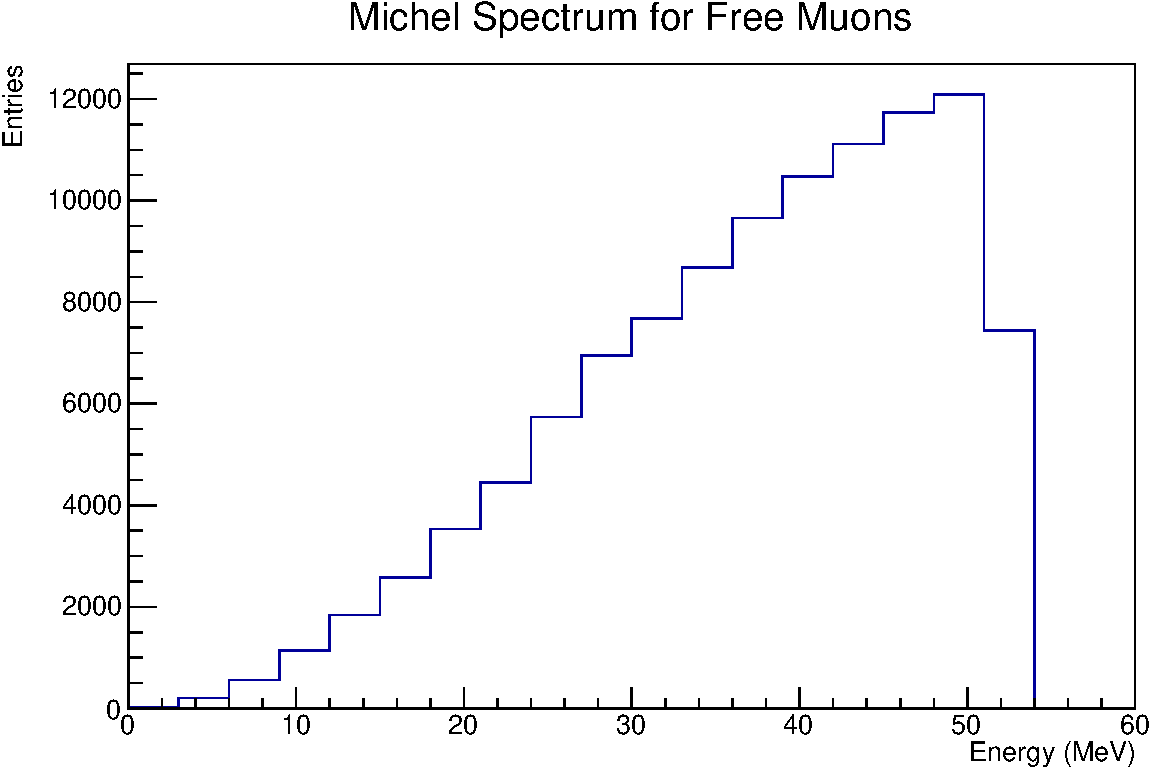
\includegraphics[width=\textwidth]{figures/michel_spec_free.pdf}
		\caption {Free Muons.}
		\label{fig:michel_spec_free}
	\end{subfigure}
	\begin{subfigure}[b]{0.7\textwidth}
		\centering
		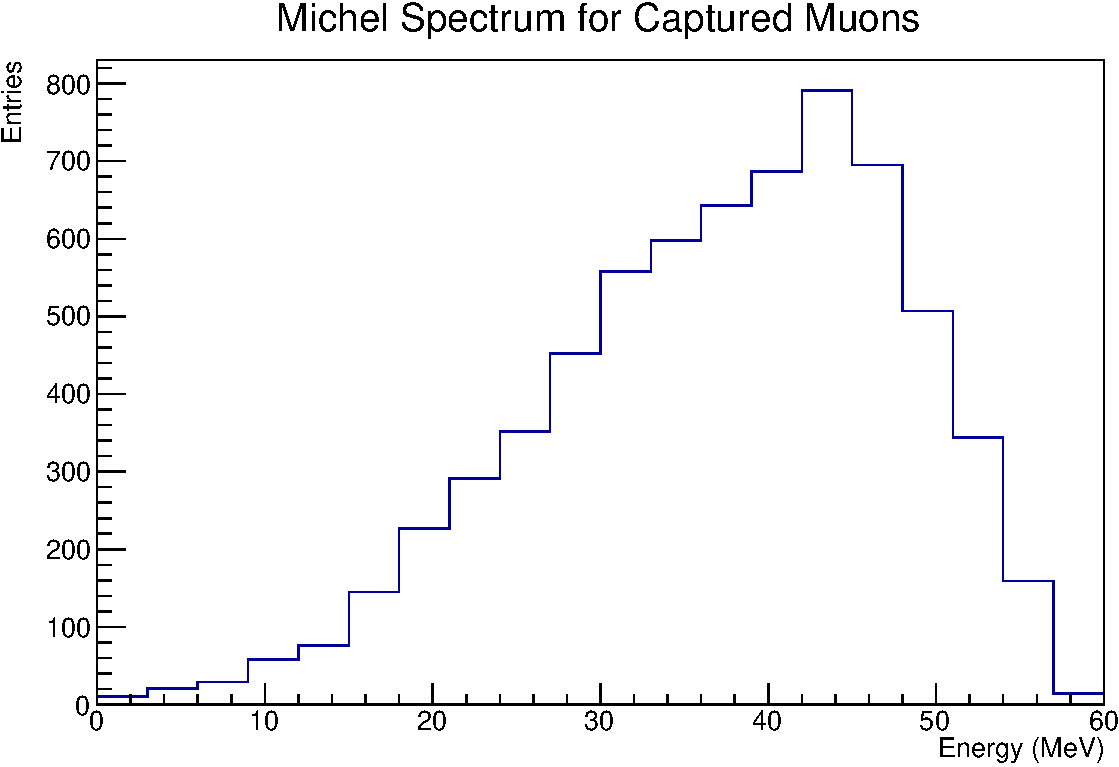
\includegraphics[width=\textwidth]{figures/michel_spec_cap.pdf}
		\caption {Captured Muons.}
		\label{fig:michel_spec_cap}
	\end{subfigure}

	\caption
	[Michel electron energy spectra in liquid argon from \protodune{} simulation.]
	{Michel electron energy spectra in liquid argon from \protodune{} simulation.}

	\label{fig:michel_spec}

\end{figure}

As discussed in chapter \ref{ch:energyloss}, the energy loss for electrons in
liquid argon passes from an ionisation dominated regime to a radiation dominated
regime in the tens of MeV region. The crossover point for this transition occurs
at around 45 MeV, very close to the peak of the Michel electron spectrum. This
leads to a unique signature for Michel electrons in liquid argon detectors, a
short ($\sim$ 5cm) track segment is surrounded by a number of small radiated 
energy deposits. Figure \ref{fig:michel_event} shows an example of a Michel 
electron candidate from \protodune{} data, along with labels of the key 
features.

\begin{figure}
	\centering
	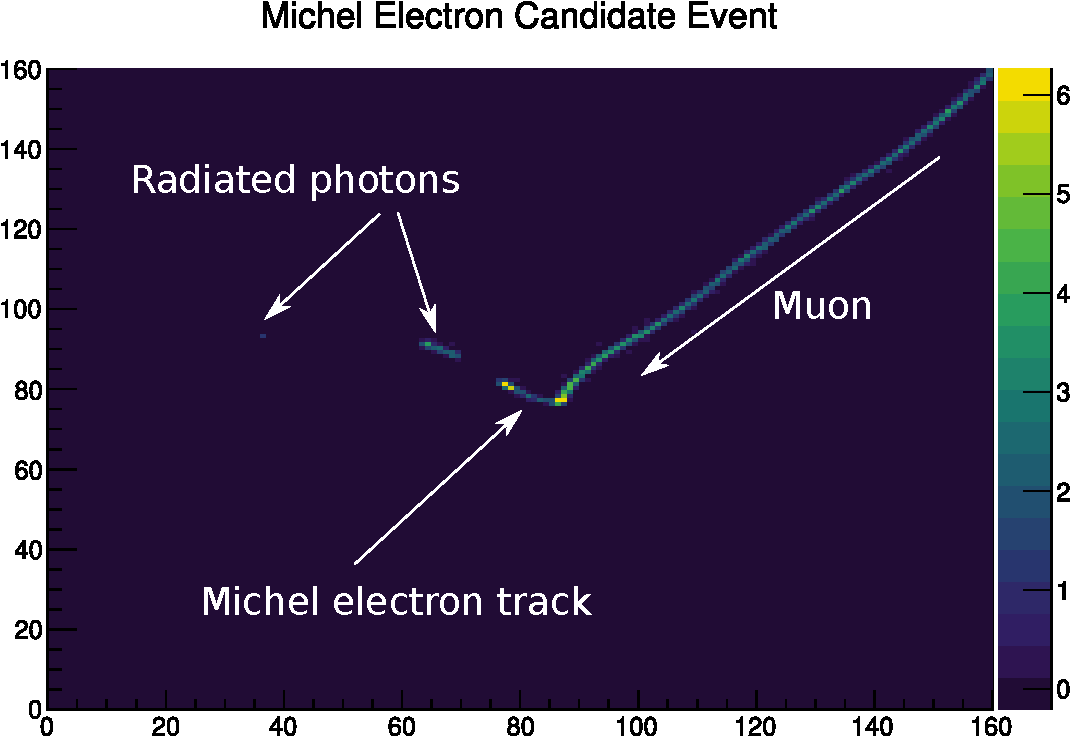
\includegraphics[width=\textwidth]{figures/michel_candidate_labelled.pdf}
	\caption
	[Michel electron candidate event from ProtoDUNE--SP data.]
	{Michel electron candidate event from ProtoDUNE--SP data. The wire vs time
	data in the region of the Michel electron event is shown.  The incoming muon,
	initial Michel electron track, and energy depositions from radiated photons
	have been labelled.}
	\label{fig:michel_event}
\end{figure}

One of the main challenges for Michel electron reconstruction in liquid argon is
to successfully associate the radiated energy depositions back to the initial
Michel electron once they have produced ionisation in the detector. Photons have
a radiation length of around 20--30 cm in liquid argon which is many times
larger than the size of the typical track--like part of the event, around 5 cm. 
Figure \ref{fig:photon_spec} shows the spectrum of radiated photons from Michel 
electron events in \protodune{} simulation alongside the photon multiplicity 
as a function of Michel electron energy. While most of the radiated photons 
only carry a small fraction of the Michel electrons energy, in some cases a 
single radiated photon can carry a significant fraction of the electron 
energy. In addition, around the peak of the Michel electron spectrum ($\sim$
45 MeV) there is a high photon multiplicity and a large spread in the
multiplicity distribution. The combination of these effects leads to a
significant spread in the fraction of radiated energy for Michel electron
events.

\begin{figure}

	\centering

	\begin{subfigure}[b]{\textwidth}
		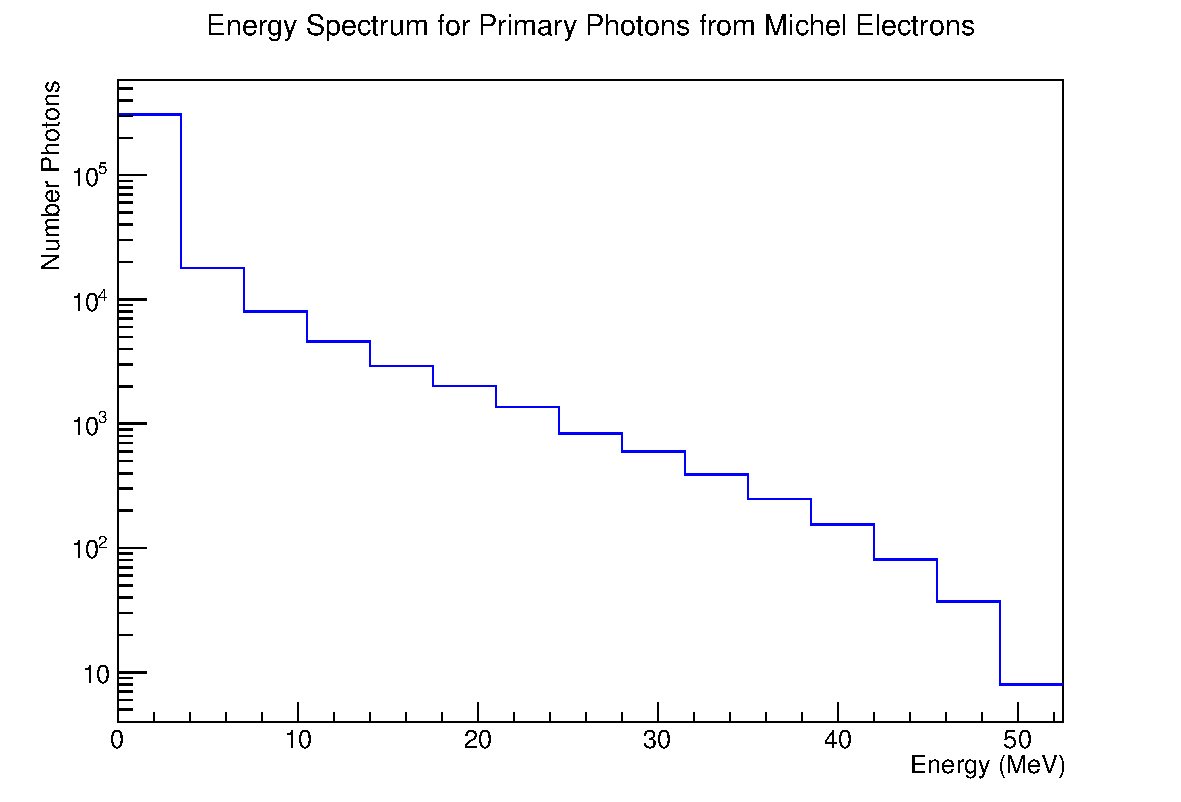
\includegraphics[width=\textwidth]{figures/photon_spec.pdf}
		\caption{Energy spectrum of radiated photons from Michel electron events.}
		\label{fig:photon_spec}
	\end{subfigure}

	\vspace{5mm}

	\begin{subfigure}[b]{\textwidth}
		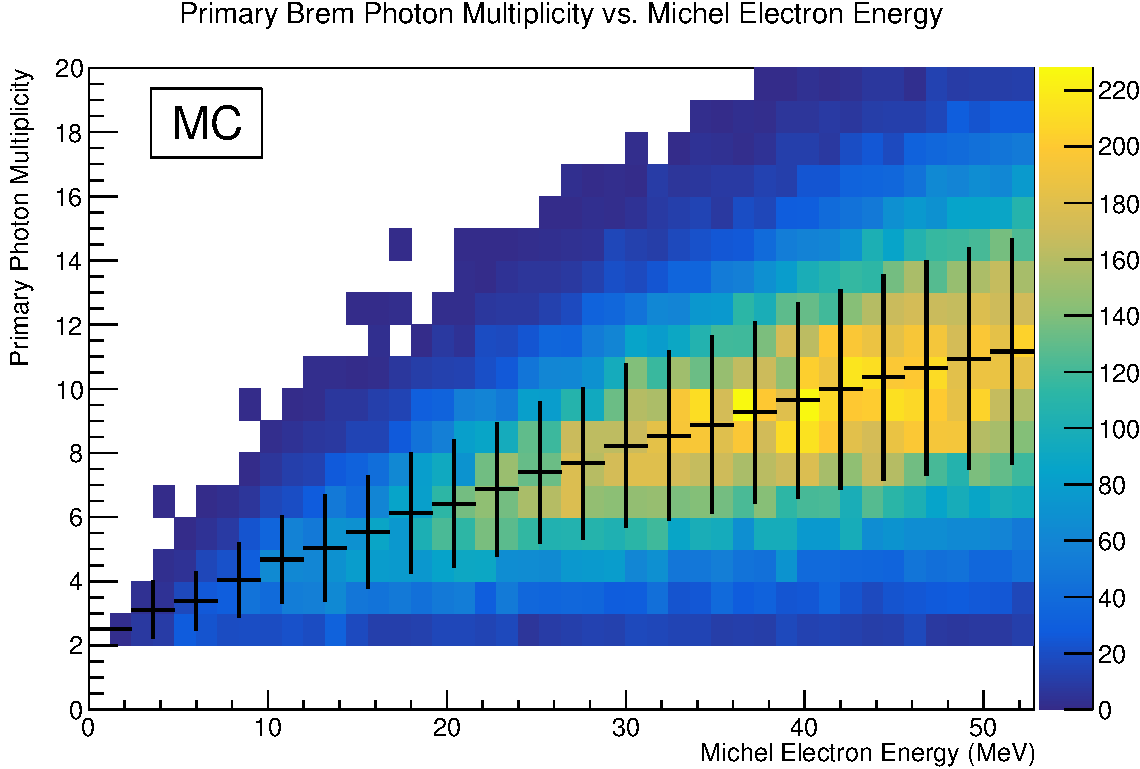
\includegraphics[width=\textwidth]{figures/photon_mult.pdf}
		\caption{Photon multiplicity as a function of true Michel electron energy.
		The distribution is overlaid with a profile of the mean of the distribution,
		the error bars on the profile represent the width of the distribution.}
		\label{fig:photon_mult}
	\end{subfigure}

	\caption
	[Properties of radiated energy deposits from Michel electrons.]
	{Properties of radiated energy deposits from Michel electrons in \protodune{}
	simulation.} 

	\label{fig:photon_prop}

\end{figure}

The energy which is lost into radiated photons is only visible once the photons
interact in the argon to produce secondary electrons which then ionise the
argon. These secondary electrons are scattered over large angles and distances
in the detector when compared to the short Michel electron track, the spatial 
distribution of secondary electrons is shown in Figure \ref{fig:photon_geom}.
This shows that the radiated energy deposits are spread over a large area, when
compared to the size of the initial Michel electron track. Therefore, any 
reconstruction algorithm hoping to recover the radiated energy, will 
need to use data from a relatively large volume in order to maximise energy
recovery.
\begin{figure}
	\centering
	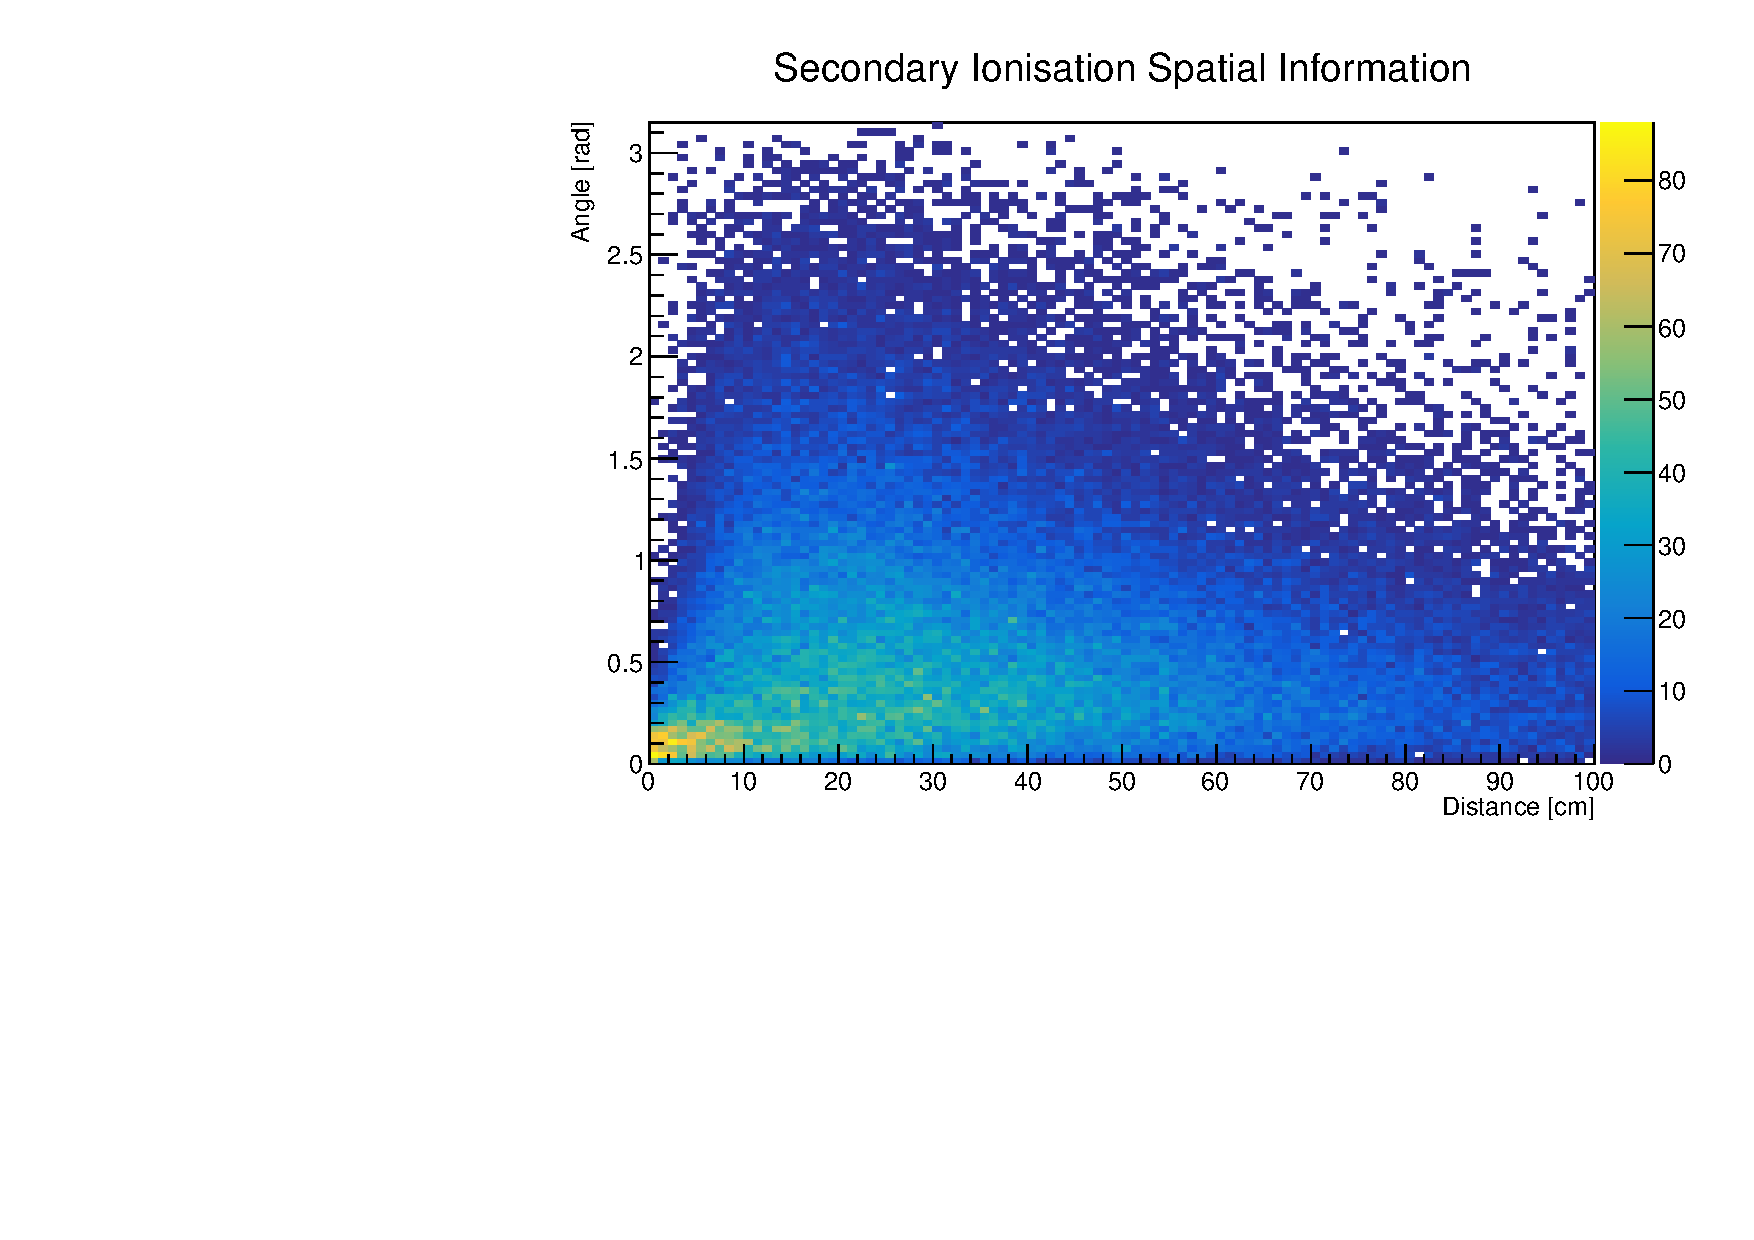
\includegraphics[width=\textwidth]{figures/photon_geom.pdf}
	\caption
	[Spatial distribution of radiated ionisation deposits.]
	{Spatial distribution of radiated ionisation deposits. This plot shows a
	2D histogram of the distance and angle of each radiated energy deposition 
	from the primary Michel electron track.}
	\label{fig:photon_geom}
\end{figure}

To highlight the impact of the radiated energy deposits we can consider the 
results of perfect energy reconstruction in two cases:
\begin{itemize}
	\item Only considering the Michel electron track.
	\item Considering all ionisation energy within some radius and angle of the 
		Michel electron track.
\end{itemize}
Figure \ref{fig:michel_track_only} illustrates the considerable increase in energy
collected if radiated energy is considered. The distribution is significantly
narrower and much more energy is recovered when considering the energy deposited
within a sphere of height $40\mbox{ cm}$ and angle 30\textdegree of the Michel 
electron vertex. In addition, the fraction of energy recovered as a function of
Michel electron energy has a more linear distribution for a collection radius of
40 cm.
\begin{figure}
	\centering

	\begin{subfigure}[b]{\textwidth}
		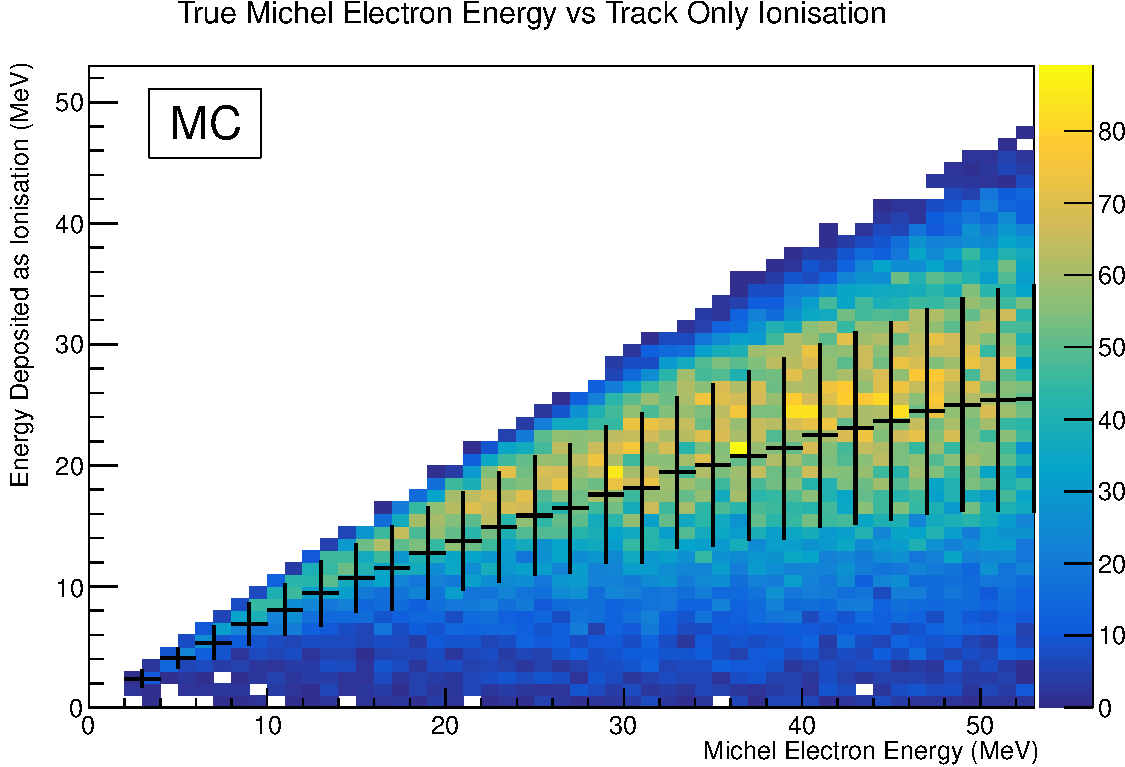
\includegraphics[clip, trim = 0cm 0cm 0cm 1cm, width=\textwidth]{figures/michel_track_only.pdf}
		\caption
		[Initial Michel electron track only.]
		{True collected ionisation energy from the initial Michel electron track
		only.}
		\label{fig:track_only}
	\end{subfigure}

	\vspace{5mm}

	\begin{subfigure}[b]{\textwidth}
		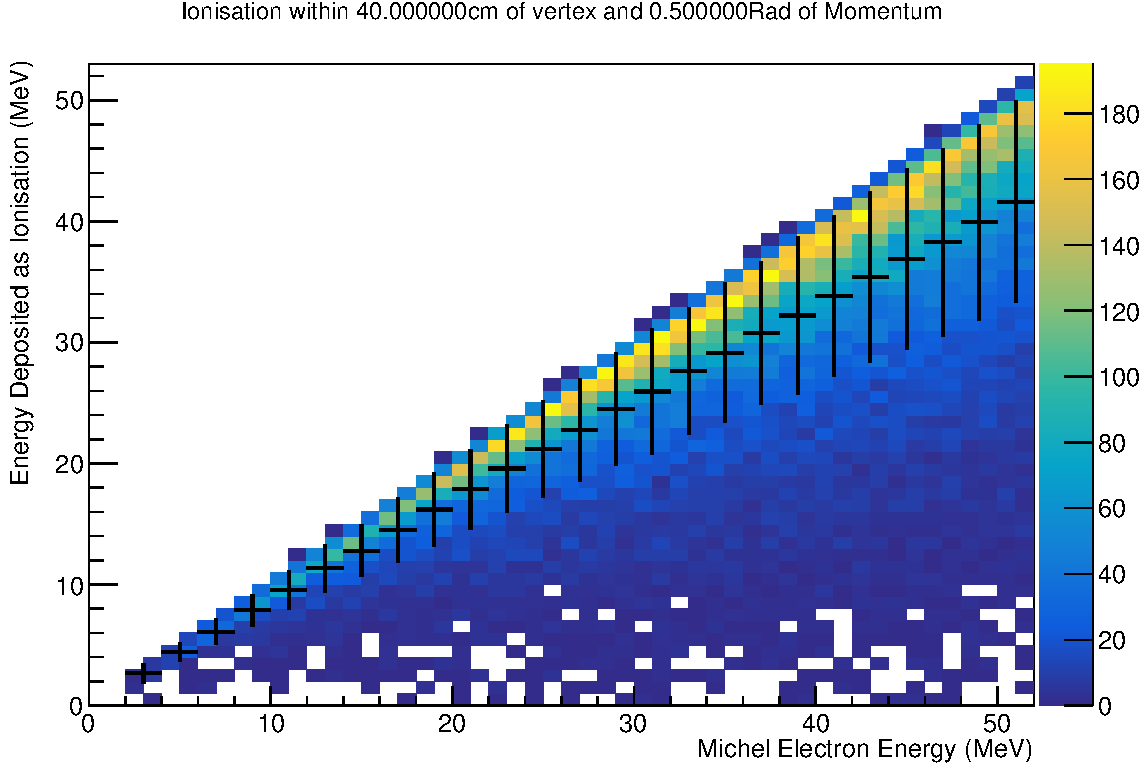
\includegraphics[clip, trim = 0cm 0cm 0cm 1cm, width=\textwidth]{figures/cone_reco.pdf}
		\caption
		[Ionisation withing a 40 cm cone at $30^\circ$ opening angle.]
		{True collected ionisation energy from the initial Michel electron track,
		and any radiated ionisation within a 40 cm cone at a $30^\circ$ opening
		angle of the initial Michel electron track.}
		\label{fig:cone_reco}
	\end{subfigure}

	\caption
	[Available ionisation energy vs true Michel electron energy.]
	{2D histograms of the true collected ionisation energy vs the true Michel
	electron energy in \protodune{} simulation.}

	\label{fig:michel_track_only}

\end{figure}

The average fractional energy recovery as a function of collection radius is
shown in Figure \ref{fig:frac_v_radius}, where the error bars represent the RMS
of the distribution. By increasing the collection radius from 0 cm to 40cm, 
the average energy recovered is increased from 57\% to 87\%. The RMS of the
fractional energy recovered reduces slightly from 20\% to 16\% across this
range. Therefore, the spread in the fraction of energy recovered is reduced 
from 35\% to 18\%. 
\begin{figure}
	\centering
	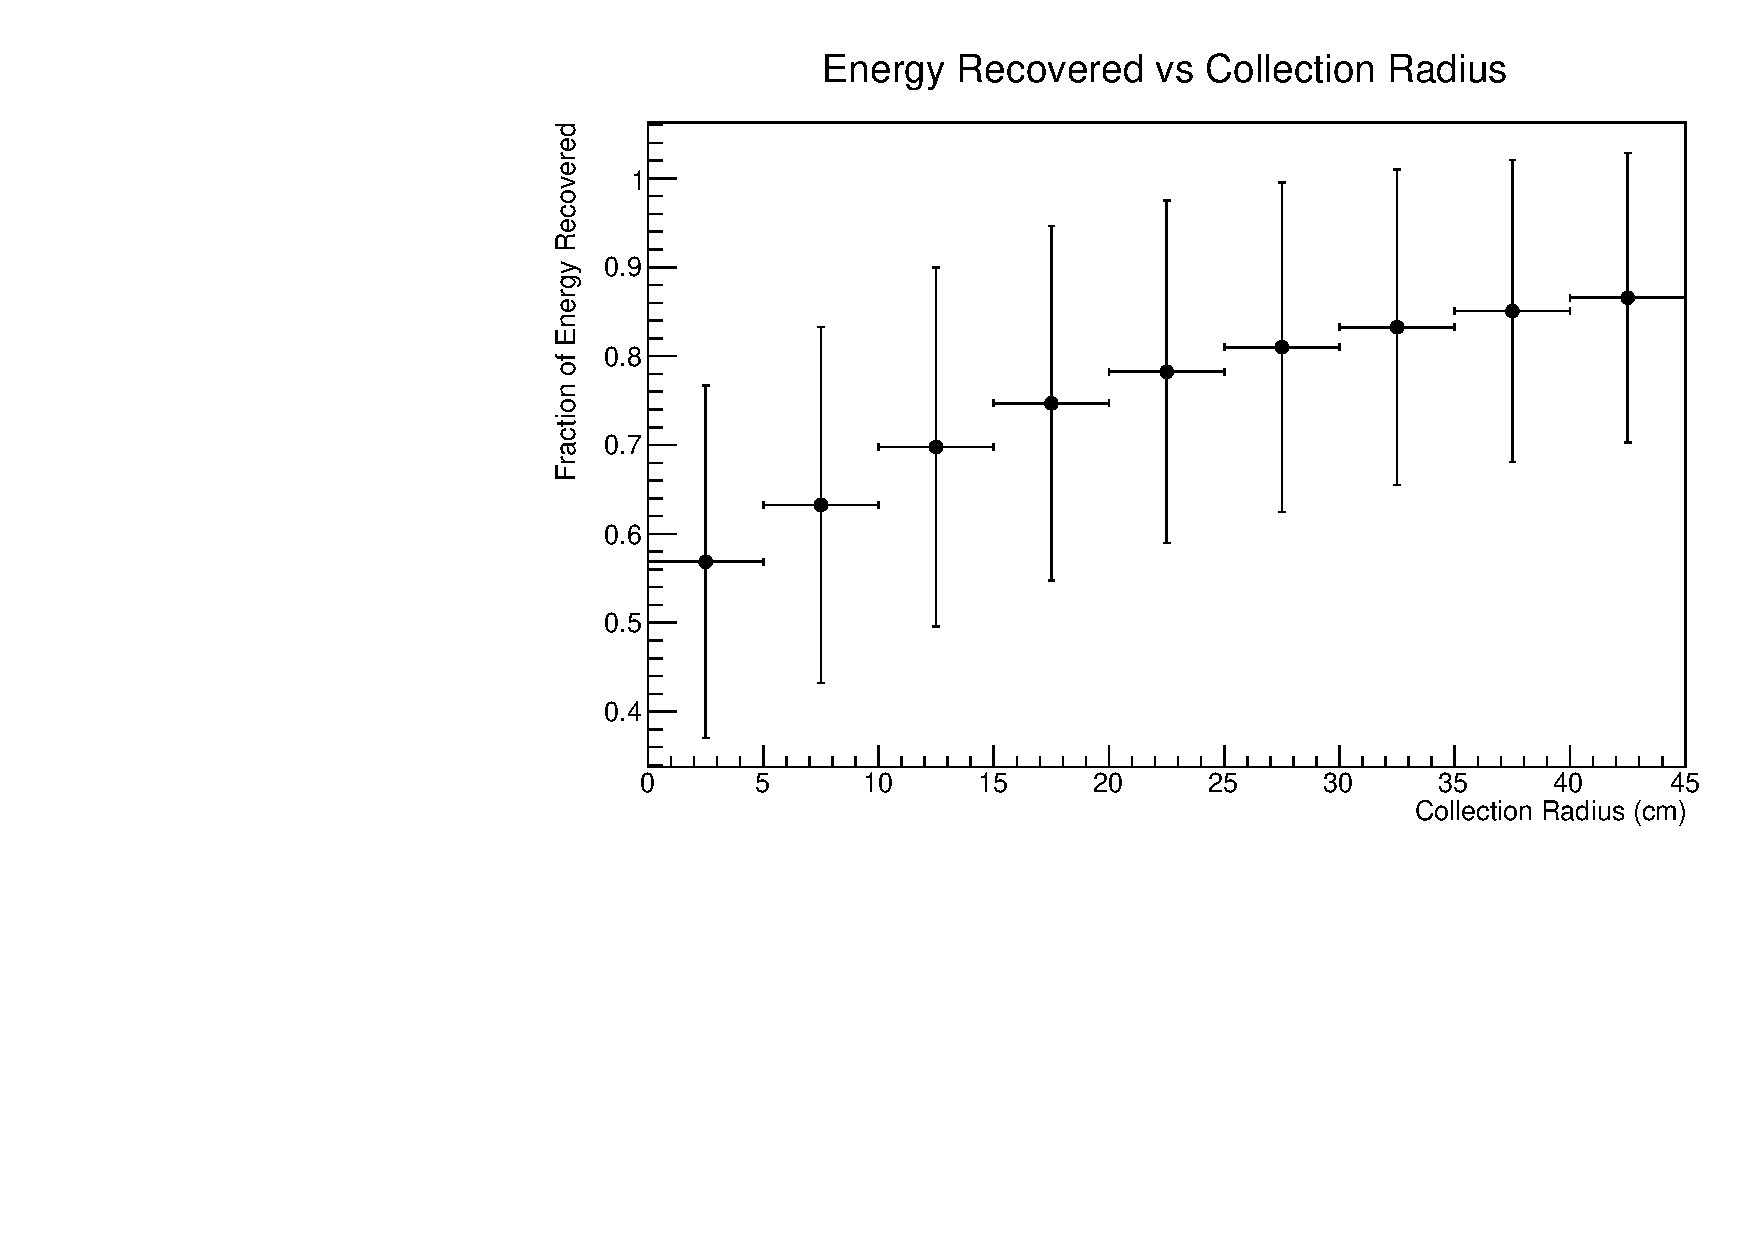
\includegraphics[width=\textwidth]{figures/energy_recovery_v_radius.pdf}
	\caption
	[Fraction of Michel electron energy collected vs collection radius.]
	{Fraction of Michel electron energy collected as ionisation vs collection 
	radius.}
	\label{fig:frac_v_radius}
\end{figure}

Increasing the collection radius beyond around 30--40 cm gives minimal
improvement in the fractional energy recovery from ionisation. This can been
seen in Figure \ref{fig:40_v_80}, which shows the total true ionisation energy
collected for the case of a 40 cm collection radius and an 80 cm collection
radius. While increasing the collection radius does not significantly increase
the collected ionisation, it is likely to impact the purity and efficiency of 
reconstruction algorithms. Therefore, the energy reconstruction algorithm 
discussed in this chapter considers a 40 cm collection radius when collecting 
radiated energy deposits.
\begin{figure}
	\centering
	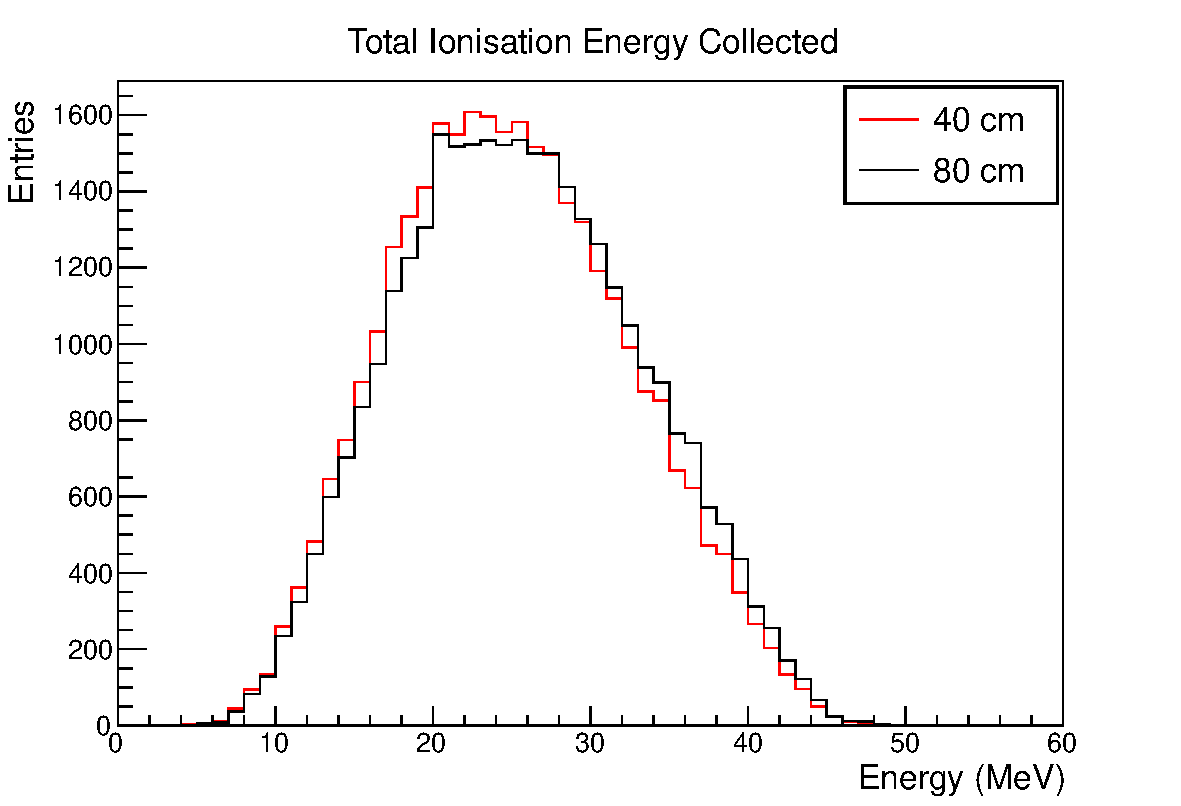
\includegraphics[width=\textwidth]{figures/40_v_80.pdf}
	\caption
	[Total true ionisation energy recovered for a 40 cm collection radius, and an
	80 cm collection radius.]
	{ Total true ionisation energy recovered for a 40 cm collection radius, and an
	80 cm collection radius. }
	\label{fig:40_v_80}
\end{figure}

The MC study presented here highlights the importance of radiated energy
deposits in Michel electron and other low--energy electron events. Based on
these results it is clear that to minimise energy uncertainties for these events
it is important to maximise the amount of energy collected from radiated 
photons. The rest of this chapter will discuss an algorithm which was developed 
to tackle this problem, and it's application on Michel electron events in 
\protodune{} data.

\section{Michel Electron Event Selection} \label{ME_ES}
In order to select Michel electrons in \protodune{} data, an event selection
algorithm was developed based on combining the results from the hit tagging CNN 
from the previous chapter with clustering performed by the main \protodune{} 
reconstruction framework, Pandora. 

The event selection algorithm has four steps:
\begin{enumerate}
	\item Start with all primary tracks from Pandora.
	\item Define a set of Michel electron candidates from the list of all
		daughters of the track.
	\item Find the best Michel electron candidate from the list of Michel electron
		candidates.
	\item Select events where the best Michel electron candidate passes the event
		selection cuts.
\end{enumerate}

First, the initial sample of muon candidates is defined. All tracks from the 
Pandora reconstruction chain which have been labelled as primary tracks are 
considered.

The second step defines a set of Michel electron candidates for each muon
candidate. A Michel electron candidate is any daughter of the primary Pandora
track which satisfies the following conditions:
\begin{itemize}
	\item Starts within 5 cm of the primary track endpoint.
	\item Contains a minimum of 5 reconstructed hits on the collection plane.
\end{itemize}

In the third step, the Michel electron candidates are analysed in order to 
define the best Michel electron candidate for each muon candidate. The best 
Michel electron candidate is the Michel electron candidate with the largest 
fraction of Michel--like hits based on the output of the Michel electron score 
from the CNN. A threshold of 0.9 is used to identify hits as Michel--like. In 
the case of a tie the Michel electron candidate with the most hits is chosen.

The fourth step is the final decision, which is based on the fraction of Michel
like hits in the best Michel electron candidate. Events are selected if the 
best Michel electron candidate is made up of more than 80 \% of Michel--like 
hits. Figure \ref{fig:michel_like_frac} shows a comparison of the fraction of 
Michel--like hits in Michel electron candidates for \protodune{} data and 
simulation. There is a good agreement between data and simulation. The pile--up
of events at one corresponds to Michel electron candidates where all hits were 
classified as Michel--like.
\begin{figure}
	\centering
	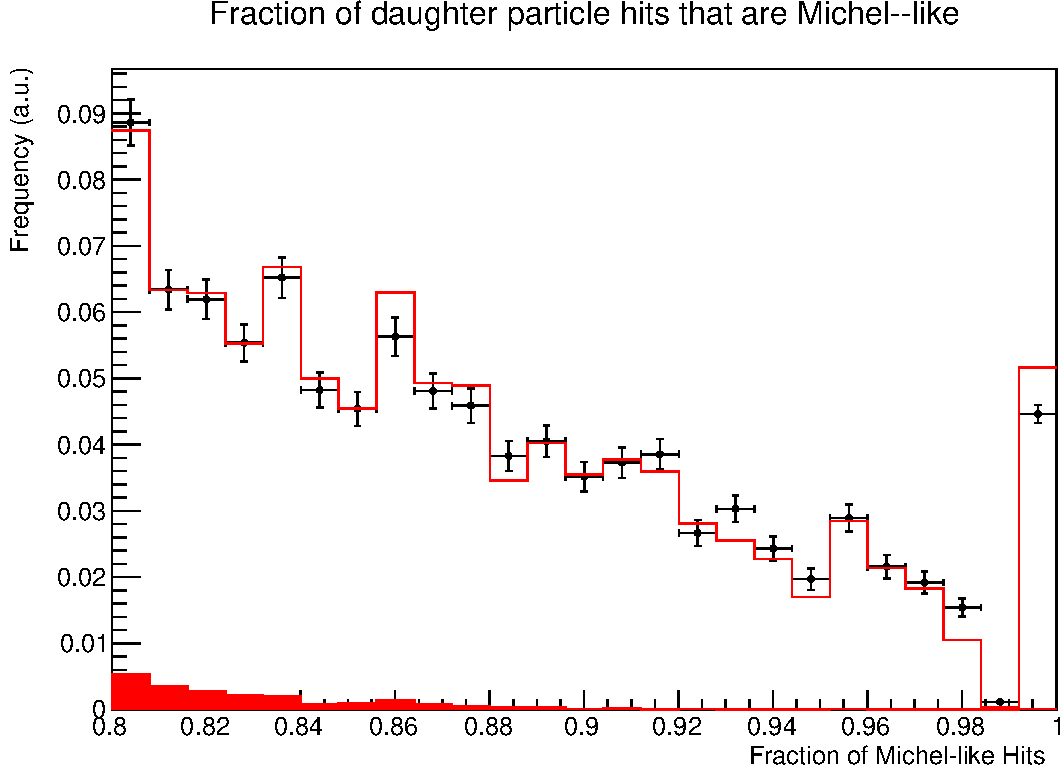
\includegraphics[width=\textwidth]{figures/michel_like_frac.pdf}
	\caption
	[Fraction of Michel--like hits in the best Michel electron candidate.]
	{Fraction of Michel--like hits in the best Michel electron candidate in data
	and simulation. The red line is the total distribution in simulation, and the 
	solid red region represents the predicted background in simulation. The black
	distribution is the results in data, where the error bars are statistical 
	only.}
	\label{fig:michel_like_frac}
\end{figure}

Based on this algorithm Michel electron events are selected with a
purity of 98\% and an overall efficiency of 6\% in \protodune{} simulation. 
Figure \ref{fig:ev_sel_eff} shows the event selection efficiency as a 
function on Michel electron energy. The efficiency is reasonably consistent
across the energy range, however, there is a significant reduction for energies
below 5 MeV. The efficiency is highest for Michel electrons in the range of 
10--40 MeV, and reduces slightly at high energies. At 40--50 MeV, around the 
peak of the Michel electron spectrum, the efficiency is around 5\%.
\begin{figure}
	\centering
	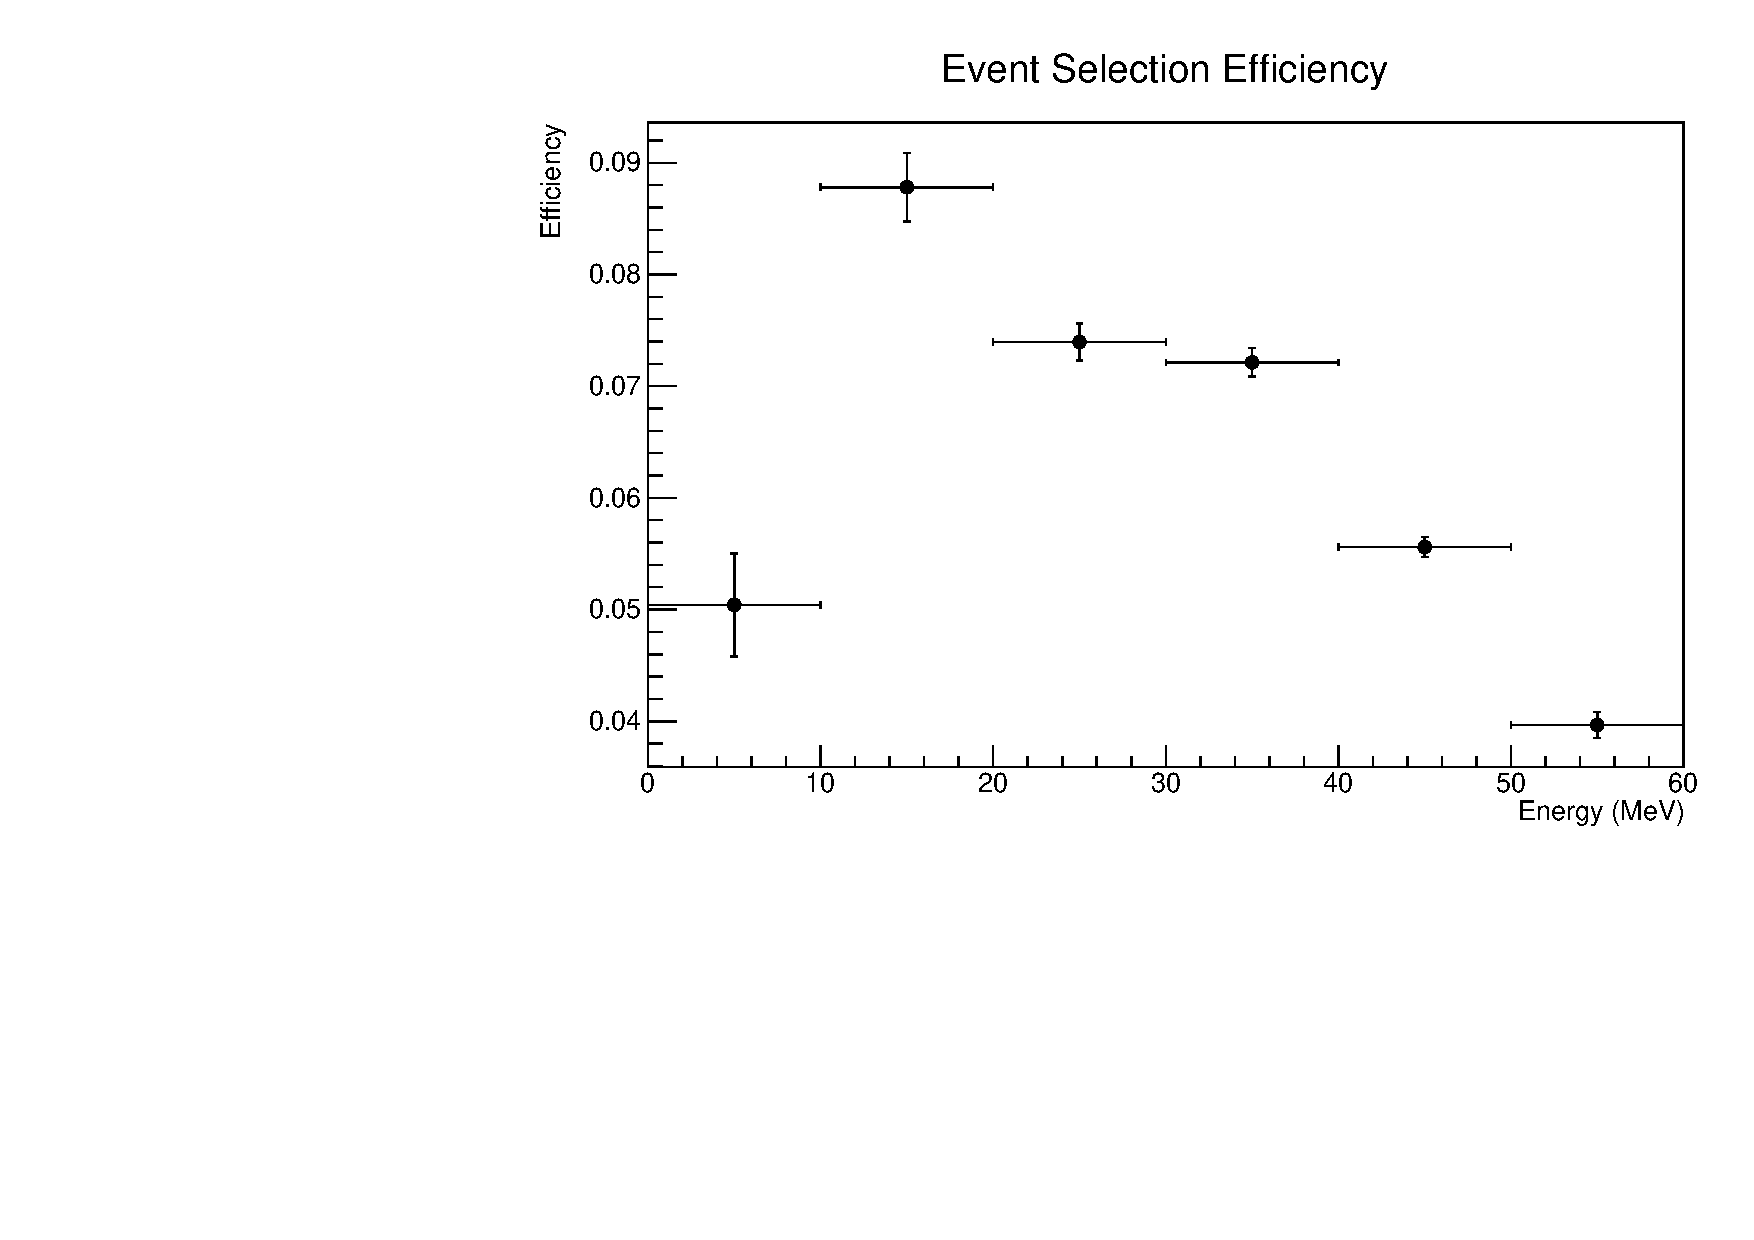
\includegraphics[width=\textwidth, height=0.68\textwidth]{figures/eff_v_energy.pdf}
	\caption
	[Efficiency of Michel electron event selection as a function of energy.]
	{Efficiency of Michel electron event selection as a function of true Michel
	electron energy in \protodune{} simulation.}
	\label{fig:ev_sel_eff}
\end{figure}

To accurately estimate the energy of hits during energy reconstruction, the 
true time of the Michel electron needs to be known. If the true time is not
known, then the drift time of the charge is unknown, and the charge attenuation
cannot be estimated. Therefore, only tracks with reconstructed true times were
considered for the Michel electron analysis. The spatial and angular
distributions of the primary muons, normalised by the number of selected 
muons, are shown in Figure \ref{fig:muon_distributions}. There is a reasonable 
agreement between data and simulation for both the spatial and angular
distributions of the primary muons.
\begin{figure}

	\centering

	\begin{subfigure}[b]{\textwidth}
		\centering
		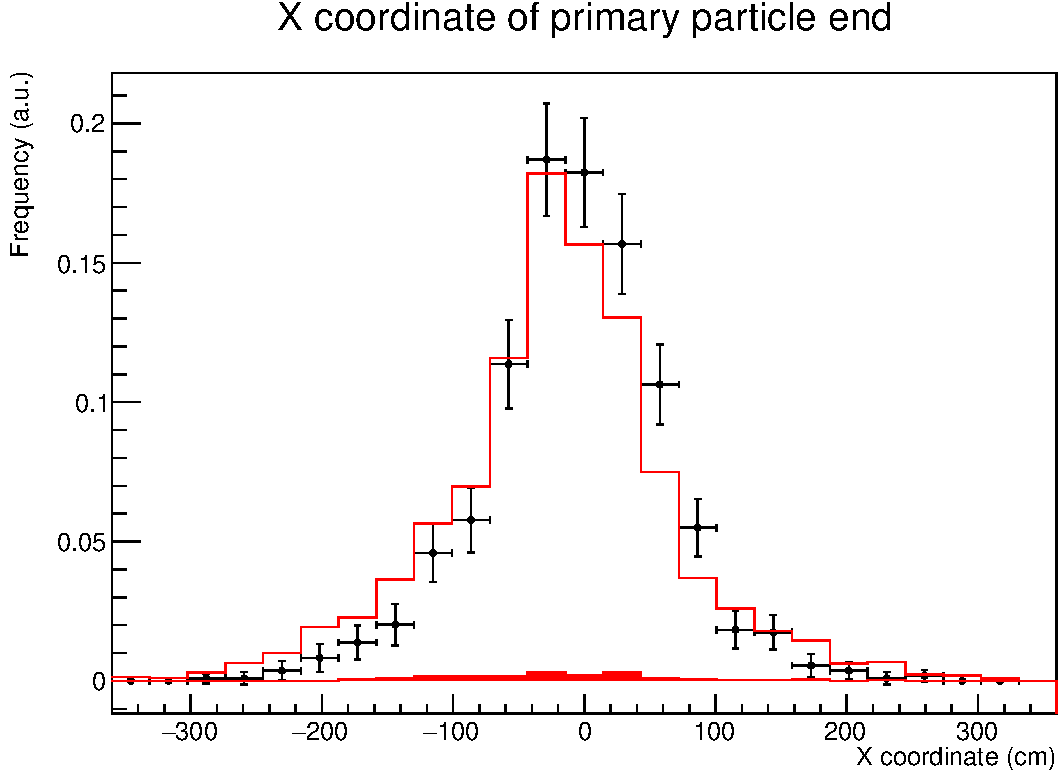
\includegraphics[width=0.49\textwidth]{figures/DataVMC_primary_EndX.pdf}
		\hfill
		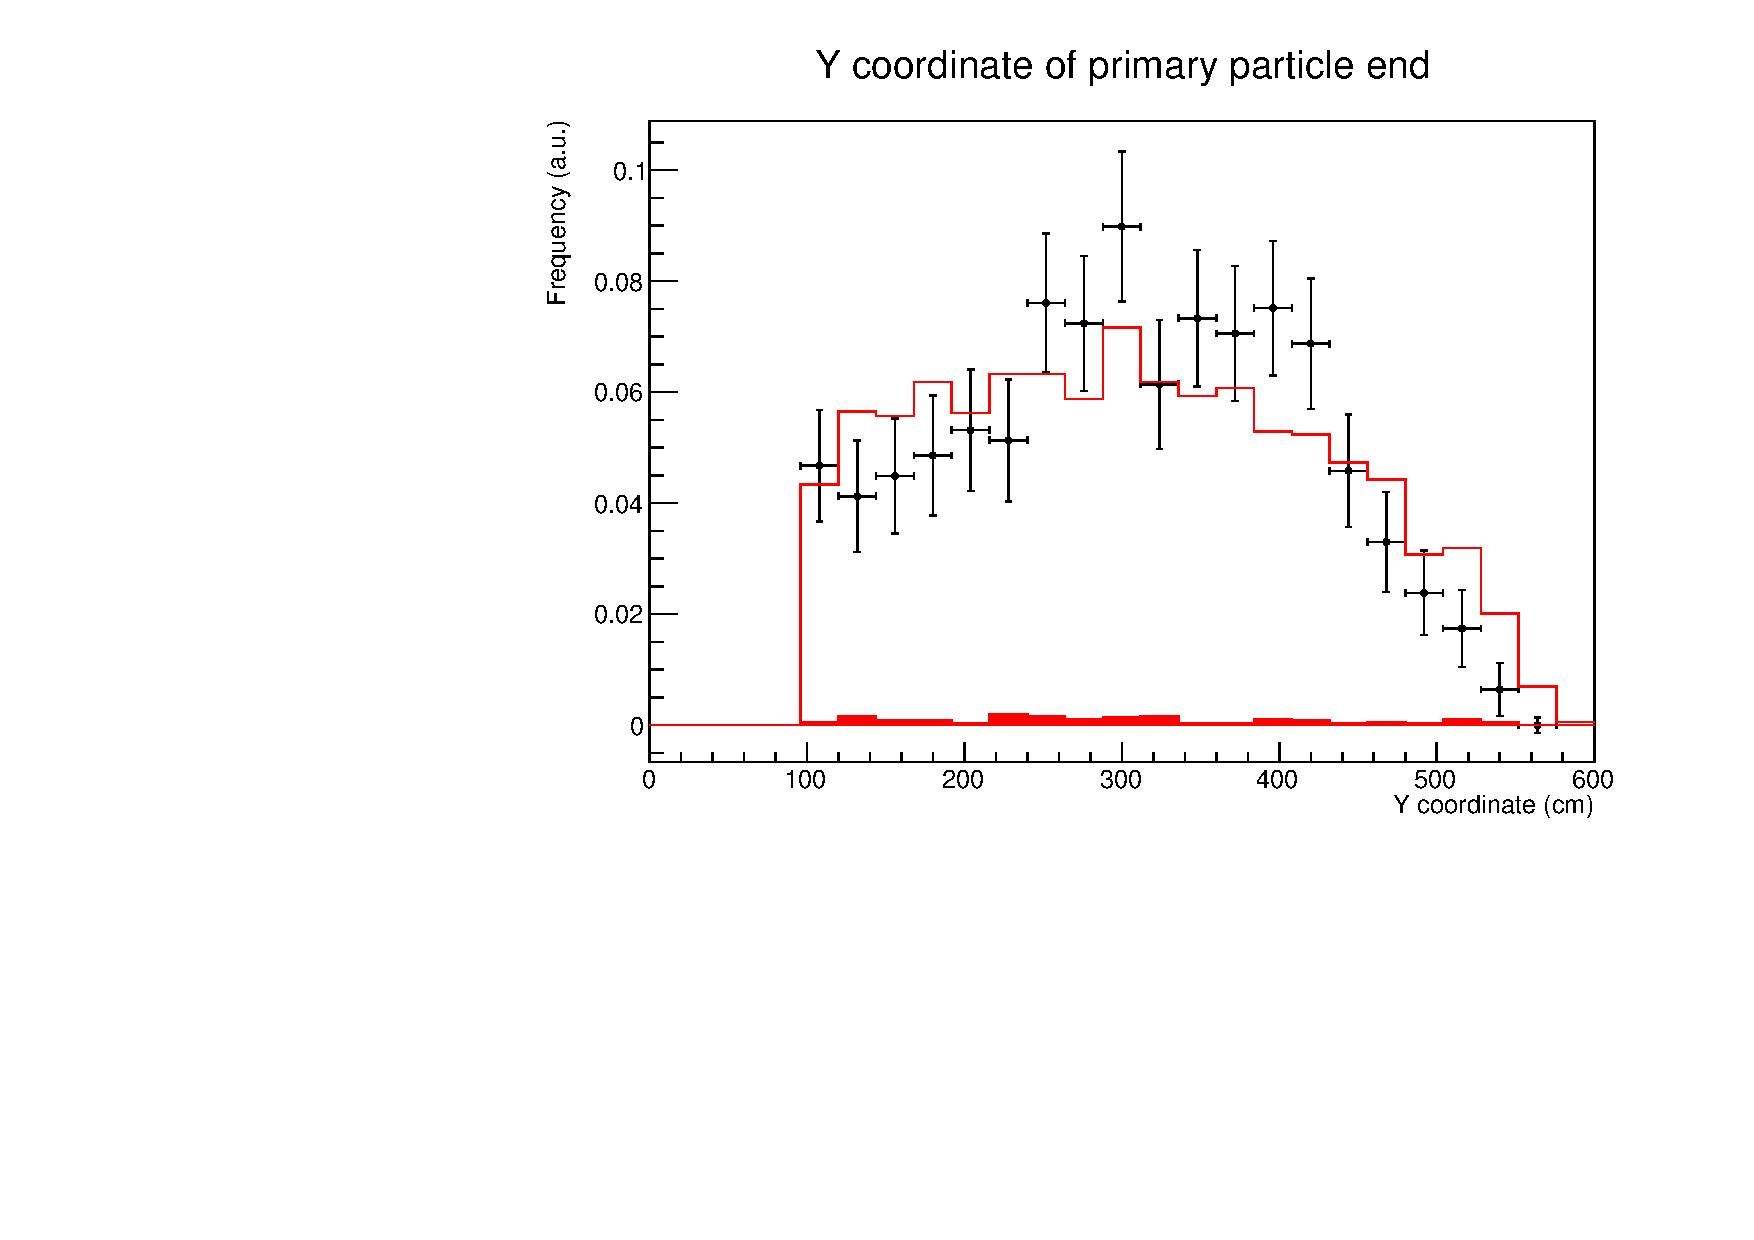
\includegraphics[width=0.49\textwidth]{figures/DataVMC_primary_EndY.pdf}
		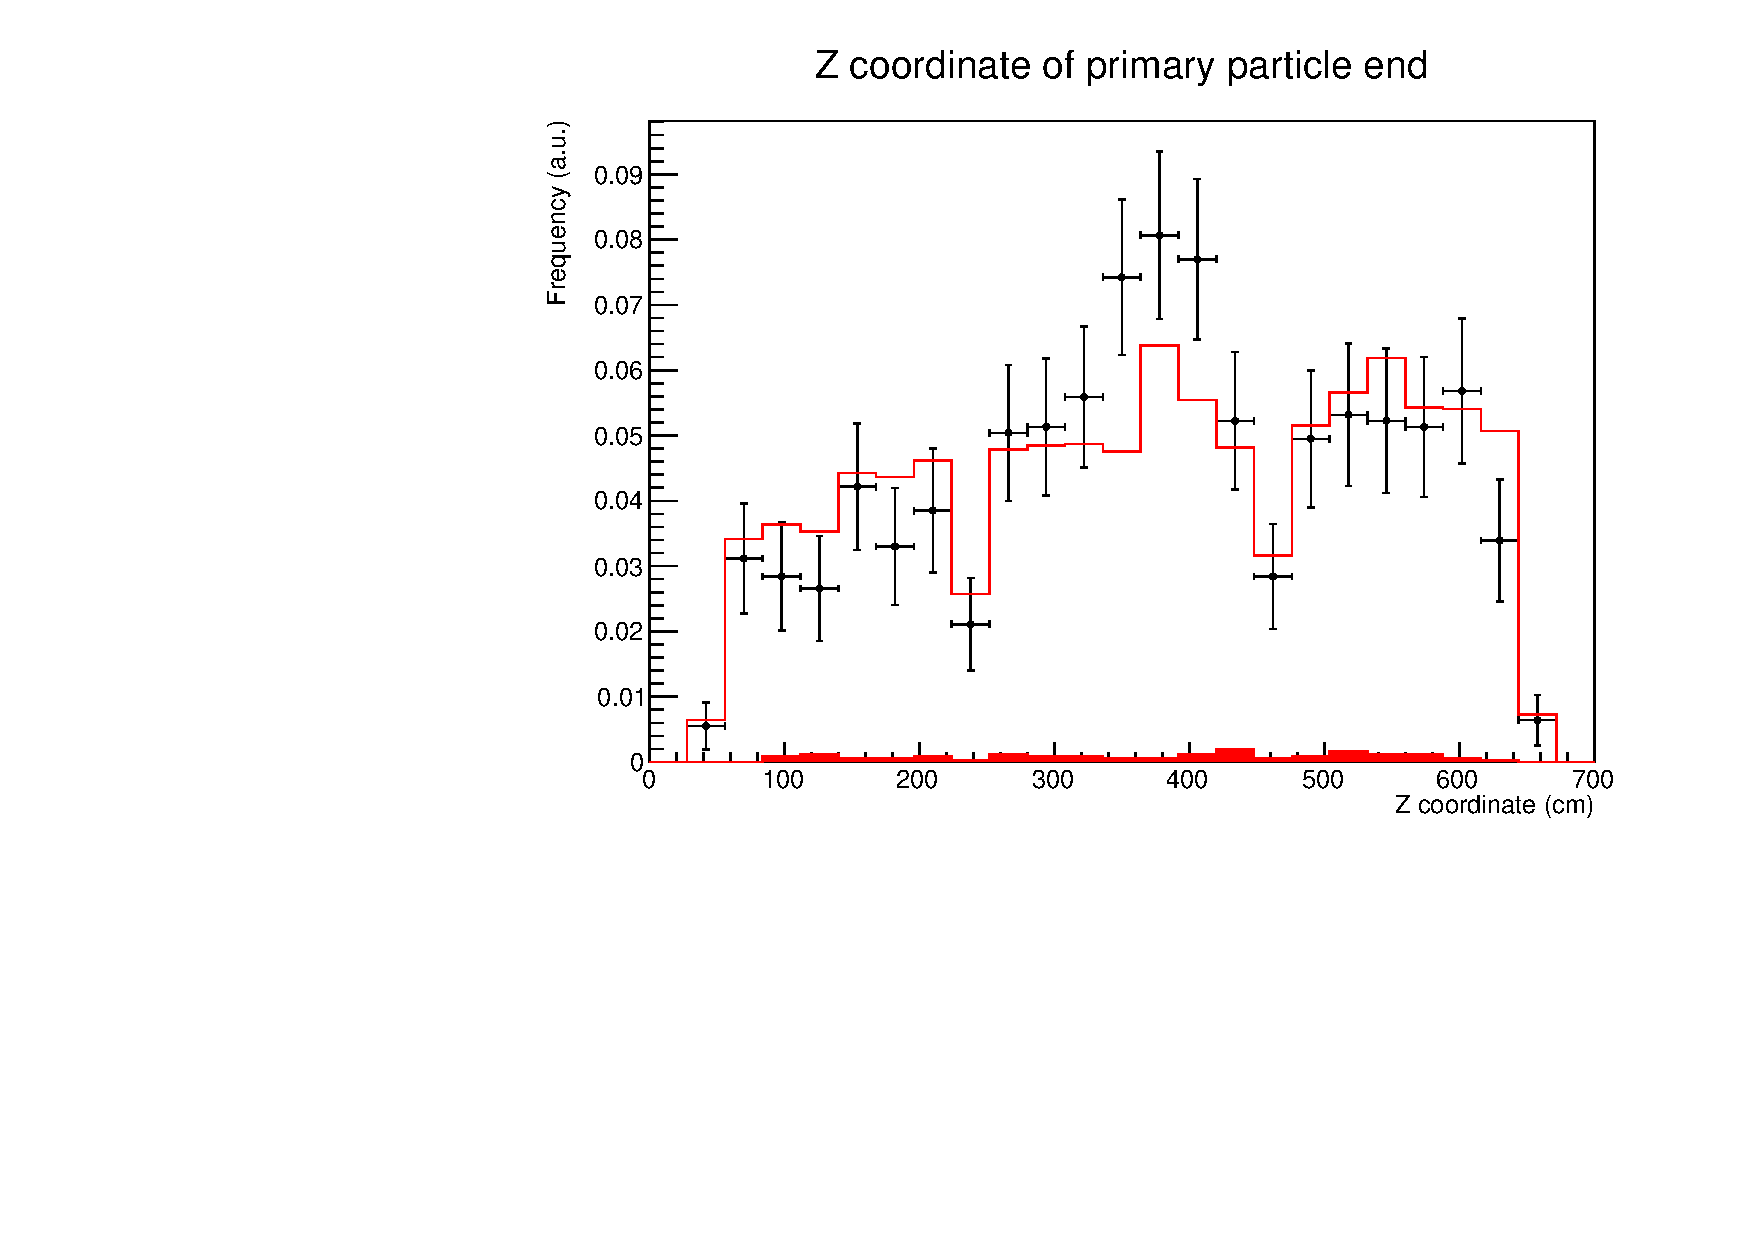
\includegraphics[width=0.49\textwidth]{figures/DataVMC_primary_EndZ.pdf}
		\caption {Primary muon end--points.}
		\label{fig:muon_endpoints}
	\end{subfigure}

	\begin{subfigure}[b]{\textwidth}
		\centering
		\vspace{1cm}
		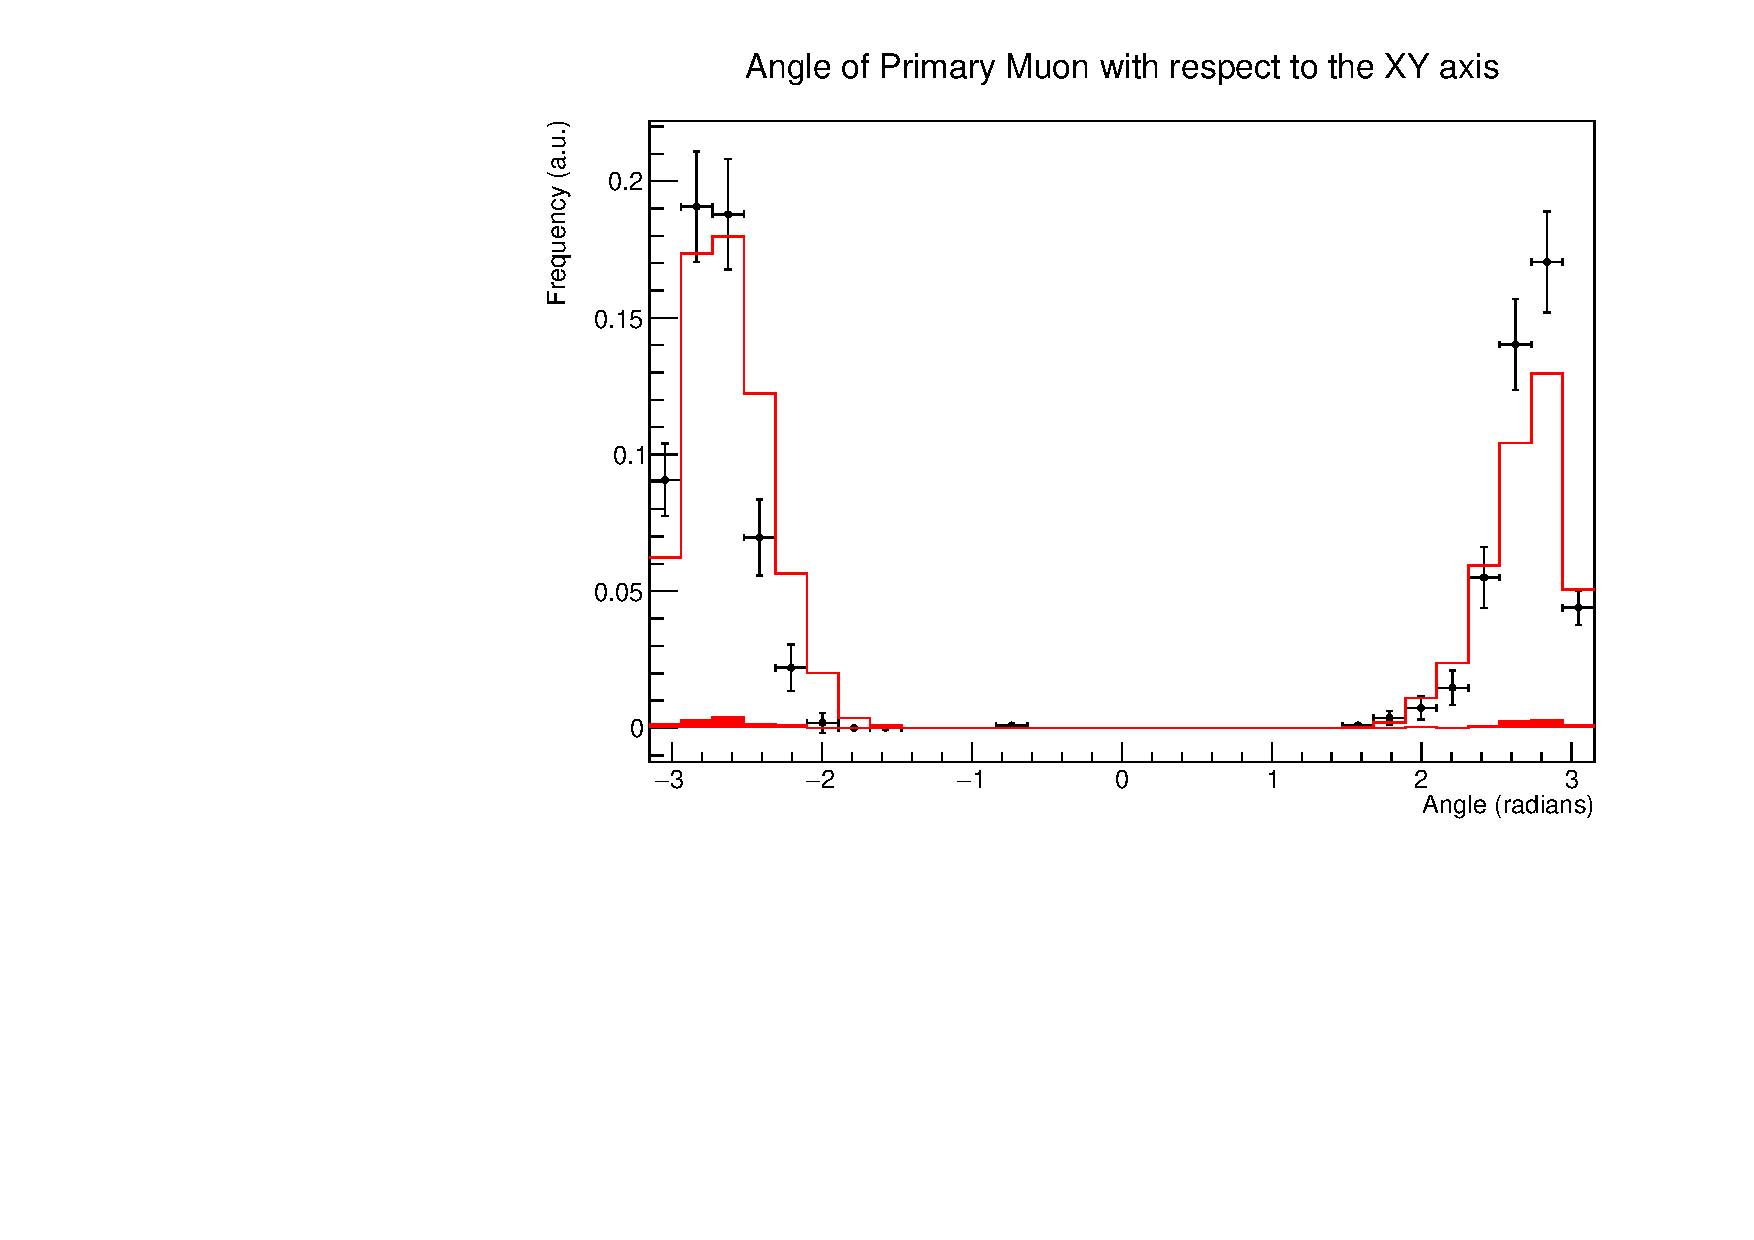
\includegraphics[width=0.49\textwidth]{figures/DataVMC_angle_xy.pdf}
		\hfill
		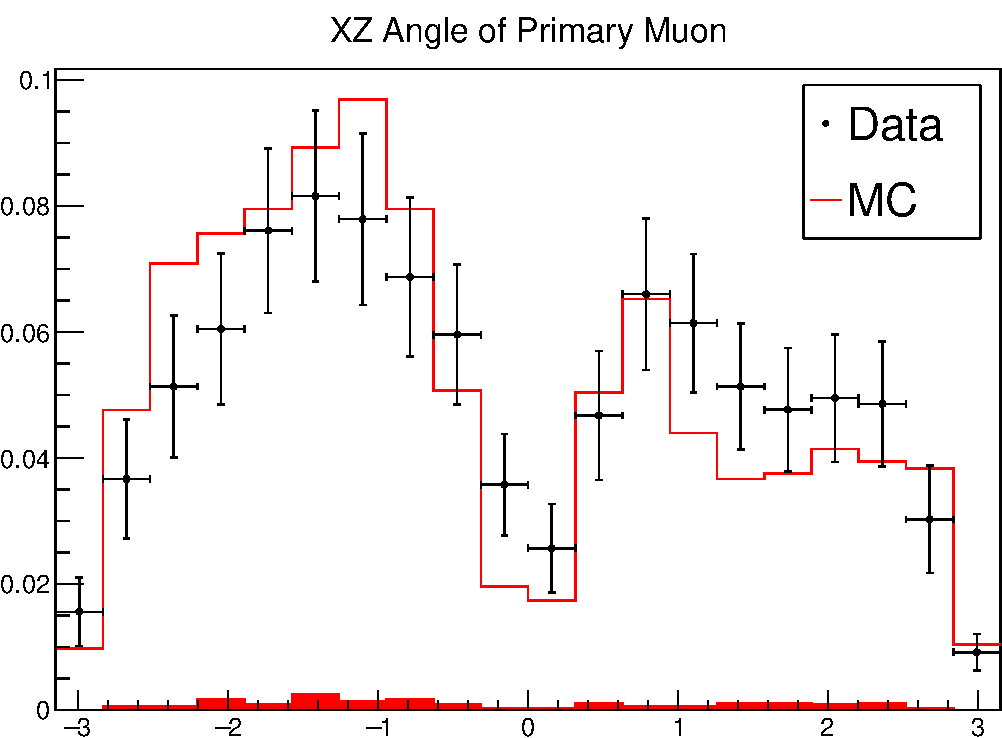
\includegraphics[width=0.49\textwidth]{figures/DataVMC_angle_xz.pdf}
		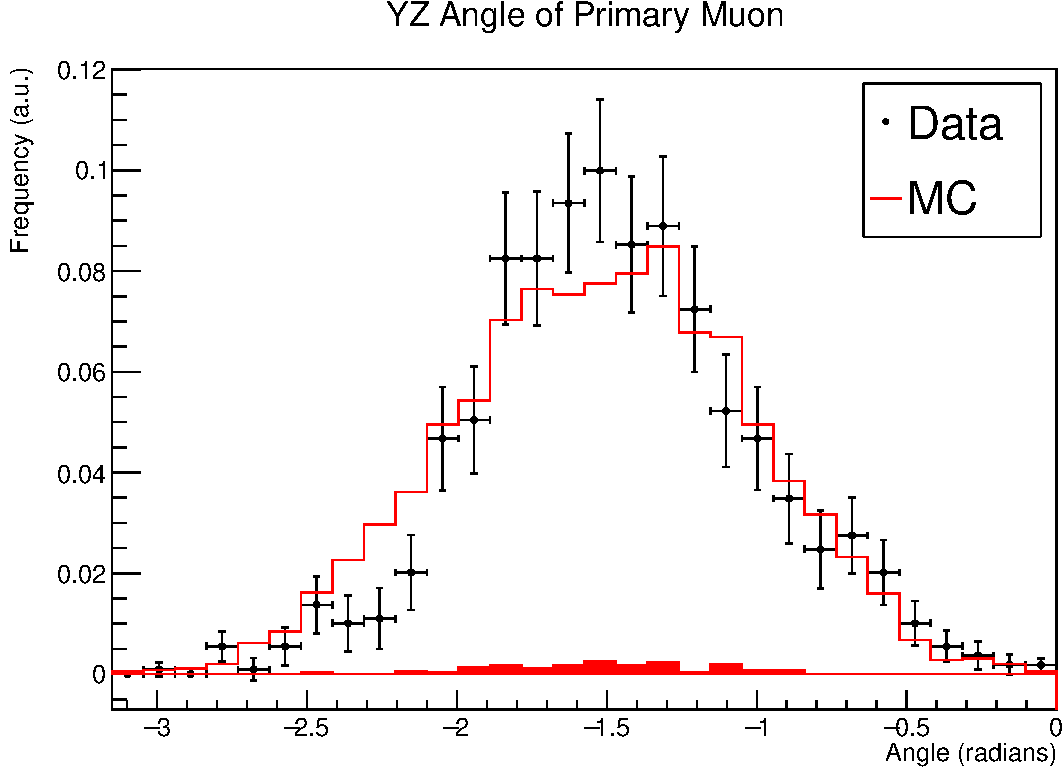
\includegraphics[width=0.49\textwidth]{figures/DataVMC_angle_yz.pdf}
		\caption {Primary muon angular distributions.}
		\label{fig:muon_angles}
	\end{subfigure}
	

	\caption
	[Spatial and angular distributions for primary muons associated with selected
	Michel electrons.]
	{Spatial and angular distributions for primary muons associated with selected
	Michel electrons.}

	\label{fig:muon_distributions}

\end{figure}

\section{Michel Electron Energy Reconstruction} \label{ME_R} 
% \begin{mccorrection}
% 	\begin{itemize} 
% 	\item U-Nets and semantic segmentation
% 	\item Algorithm outline
% 	\item Details of my U-Net
% 	\item Architecture plot
% 	\item Map examples
% 	\item Data v MC score distribution
% 	\item Reco spectrum
% 	\item NHits
% 	\item Energy per hit
% 	\item Reco geometry variables
% 	\end{itemize}
% \end{mccorrection}

To reconstruct the energy of Michel electrons in liquid argon the relevant hits
must first be selected. Once the hits are selected the ionisation energy
deposited by each hit is then reconstructed, the reconstructed energy of the 
Michel electron is the sum of the reconstructed energy of all relevant hits. In
this section we will detail a hit selection algorithm based on a type of
convolutional neural network called a U-Net, which returns hit selection maps 
for the Michel electron energy reconstruction. This algorithm is used to select 
Michel electron hits with a high purity and efficiency, the resulting 
reconstructed energy spectrum is used to estimate the energy resolution of 
\protodune{} for electrons in the tens of MeV range.

\subsection{Michel Electron Hit Tagging with U-Nets}

A U-Net is a type of convolutional neural network which is designed to perform
semantic segmentation of images, which was first developed for biomedical image
segmentation\cite{ronneberger2015u}. In semantic segmentation the goal
is to return a map of pixels which correspond to the areas of interest; the 
output of the network is the same dimension as the input with a one--to--one 
correspondence between input pixels and output pixels. The architecture used 
for the hit selection algorithm is shown in Figure \ref{fig:unet_arch}. During 
the first half of the network architecture the resolution of the output is 
decreases, this is analogous to many conventional CNN's and during this phase 
the network learns about the content of the image.  The second phase of the 
architecture allows the U-Net to rebuild the locations of different features 
within the initial image, this is achieved by passing the details of previous 
layers to the network as the resolution of the output map is slowly increased 
back to the original resolution.

In the Michel electron case, the goal of the network is to return a map of all
ionisation energy deposits which come from the Michel electron, this includes
the initial track and any secondary deposits from radiated photons. The inputs
and outputs are two dimensional images of the location of reconstructed hits
centered on the selected Michel electron. The amplitude of each input pixel is 
given by the integrated charge of any reconstructed hits within the pixel. For
the outputs the pixels have an amplitude of 1 if they contain a Michel electron
hit, and 0 otherwise. Only data from the collection plane is used because there 
is a higher signal to noise ratio on these wires. 

The $F_\beta$ metric was used as the loss function for the U--Net. This loss is
a generalised version of the $F_1$ metric discussed in Chapter
\ref{ch:chargeid}, which allows for the relative importance of precision and
recall to be tuned,
\begin{equation}
	F_\beta = \left( 1 + \beta^2\right) \frac{precision \cdot
	recall}{\left(\beta^2 \cdot precision\right) + recall}.
\end{equation}
This loss rewards the network for selecting as many correct hits as possible
(high recall), while penalising it for selecting more hits that necessary (low
precision). The $F_\beta$ score lies between 0 and 1, with a score of 1
corresponding to a perfect match. The \beta parameter was chosen to be 2, such 
that recall was considered to be more important than precision. This was found
to improve the performance, however, no rigorous optimisation of $\beta$ was
performed.

The network architecture used for the Michel electron reconstruction is shown in
Figure \ref{fig:unet_arch}. The network consists of a repeating structure which
contains the following key components:
\begin{itemize}
	\item Convolutional blocks, which contain multiple convolutional layers.
	\item Pooling layers for downscaling in the first half of the network.
	\item Residual connections and up--sampling in the second half of the network.
\end{itemize}
The convolutional blocks each contain three convolutional layers, which is 
shown in Figure \ref{fig:conv_block}. These take the form of inception 
units\cite{Szegedy2015} with Leaky ReLU activation functions, a schematic of 
the inception units is shown in Figure \ref{fig:unet_inception}. During the 
first half of the network, maximum pooling is used to downsample the size of 
the feature maps, which reduce by a factor of two in each max pooling layer. 
Then, during the second half of the network, the up--sampling layers increase 
the resolution of the feature maps by a factor of two, such that the output of 
the network has the same resolution as the input.  The residual connections 
from early layers, are combined with the up--sampled feature maps, to allow 
the network to reconstruct the location of the learned features. As with the 
CNN from the previous chapter, both dropout and early--stopping are 
implemented to prevent over--fitting.

\begin{figure}

	\centering

	\begin{tabularx}{\textwidth}{cX}
		\begin{subfigure}[b]{0.40\textwidth}
			\centering
			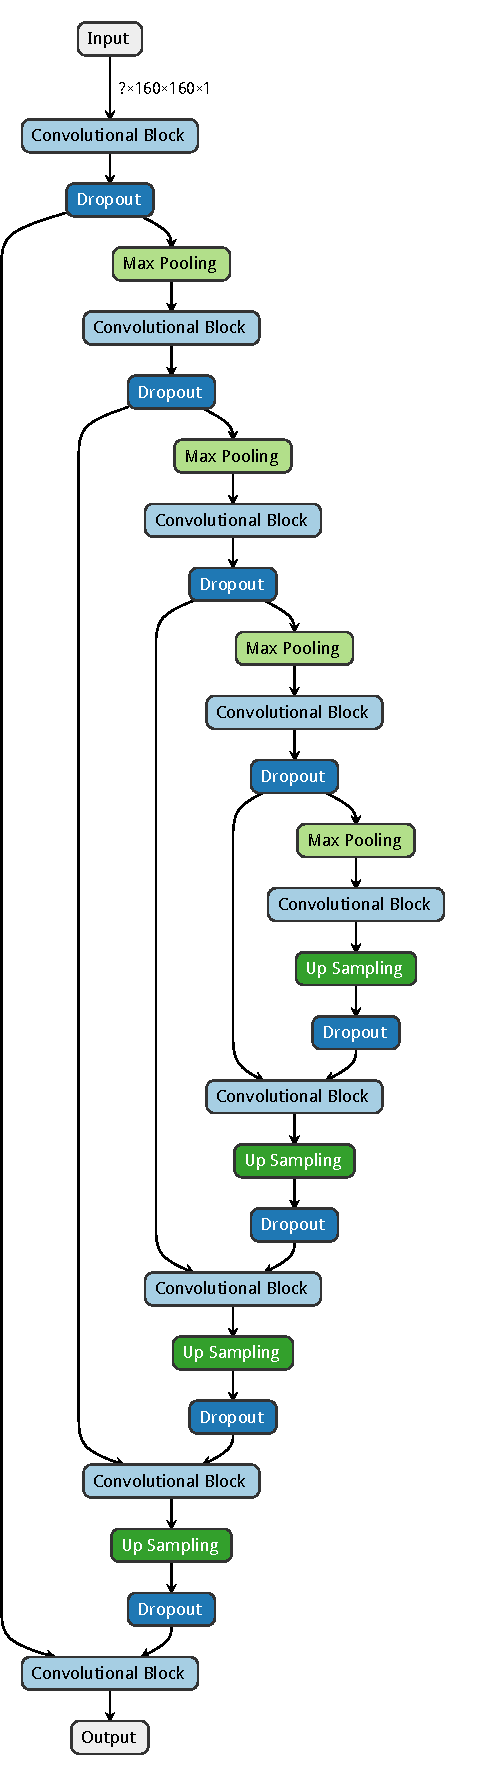
\includegraphics[height=0.90\textheight]{figures/unet_arch.pdf}
			\caption {Overall structure.}
			\label{fig:unet_structure}
		\end{subfigure}
		&
		\begin{tabular}[b]{c}
			\begin{subfigure}[b]{0.5\textwidth}
				\centering
				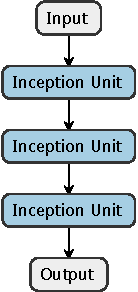
\includegraphics{figures/conv_block.pdf}
				\caption {Convolutional block.}
				\label{fig:conv_block}
			\end{subfigure} \\ 
			\vspace{10mm} \\
			\begin{subfigure}[b]{0.5\textwidth}
				\centering
				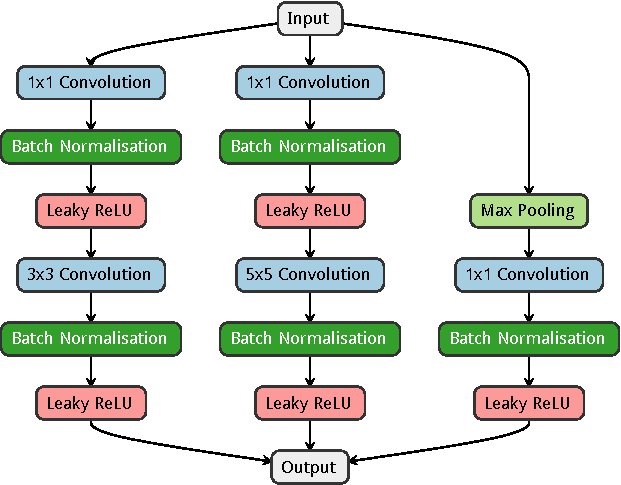
\includegraphics[width=\textwidth]{figures/inception_arch.pdf}
				\caption {Inception unit.}
				\label{fig:unet_inception}
			\end{subfigure}
		\end{tabular}
	\end{tabularx}

	\caption
	[U--Net CNN architecture used to select ionisation energy deposits.]
	{U--Net CNN architecture used to select ionisation energy deposits. 
	Visualisation adapted from the output of the Netron neural network 
	viewer\cite{netron}.}

	\label{fig:unet_arch}
\end{figure}

The datasets for the training process were generated from a full simulation of 
the \protodune{} detector under beam operation including both cosmic--ray and
beam particles. The images produced contain the location and integrated charge
for each hit within the image window. The training data is split into 
training, test, and validation sets in the ratio 80:10:10. In total around 
15,000 images used in the training, test, and validation datasets. 

As with the hit tagging CNN from the previous chapter, the training and
validation scores were monitored throughout training using TensorFlow. The
weights of the network were saved after each epoch, and the final weights were
those from the epoch before the epoch when the validation score first decreased.
Figure \ref{fig:unet_loss} shows the evolution of the loss over time, along with
a vertical line representing the loss at which the weights were chosen.
\begin{figure}
	\centering
	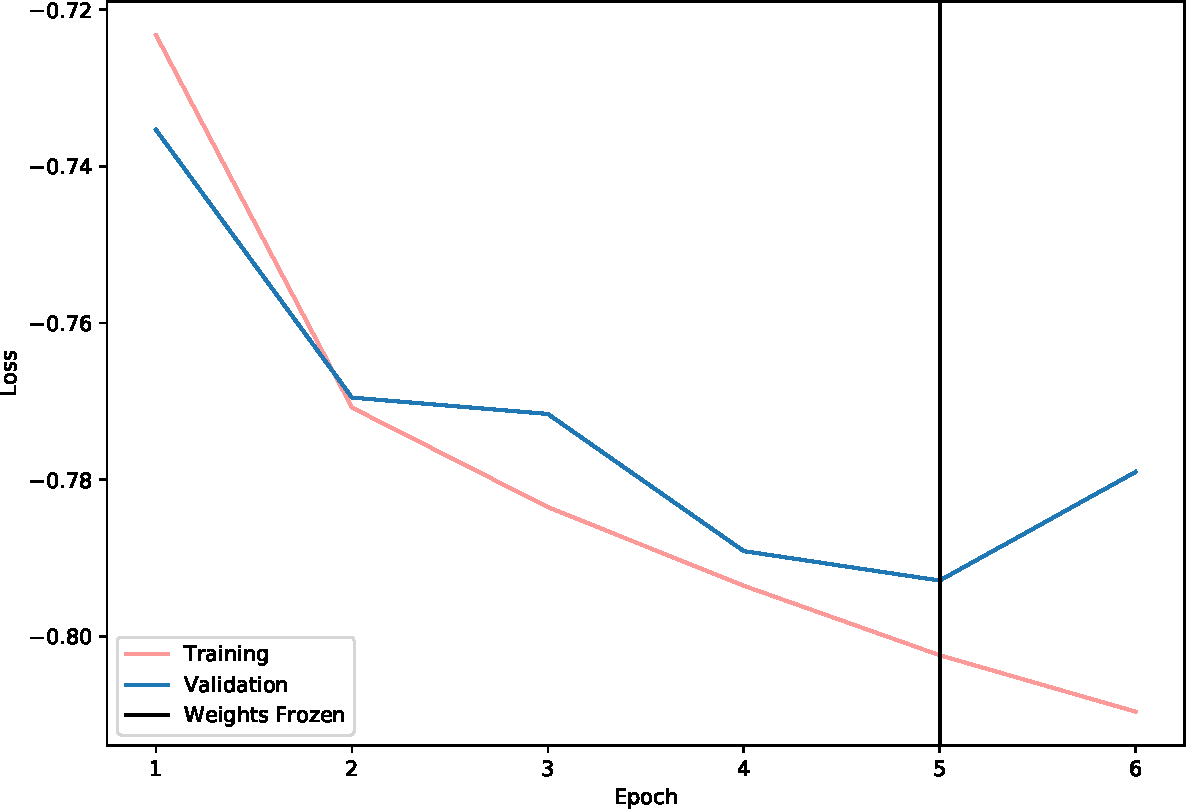
\includegraphics[width=\textwidth]{figures/unet_loss.pdf}
	\caption
	[U-Net training and validation loss as a function of epoch.]
	{U-Net training and validation loss as a function of epoch. The weights were
	frozen based on an early stopping algorithm, which is demonstrated by the
	vertical black line.}
	\label{fig:unet_loss}
\end{figure}

A demonstration of the output of the U-Net is given in Figure 
\ref{fig:unet_example} which shows the input, output, and truth images for an 
event from \protodune{} simulation.
\begin{figure}
	\centering

	\begin{subfigure}[b]{0.5\textwidth}
		\centering
		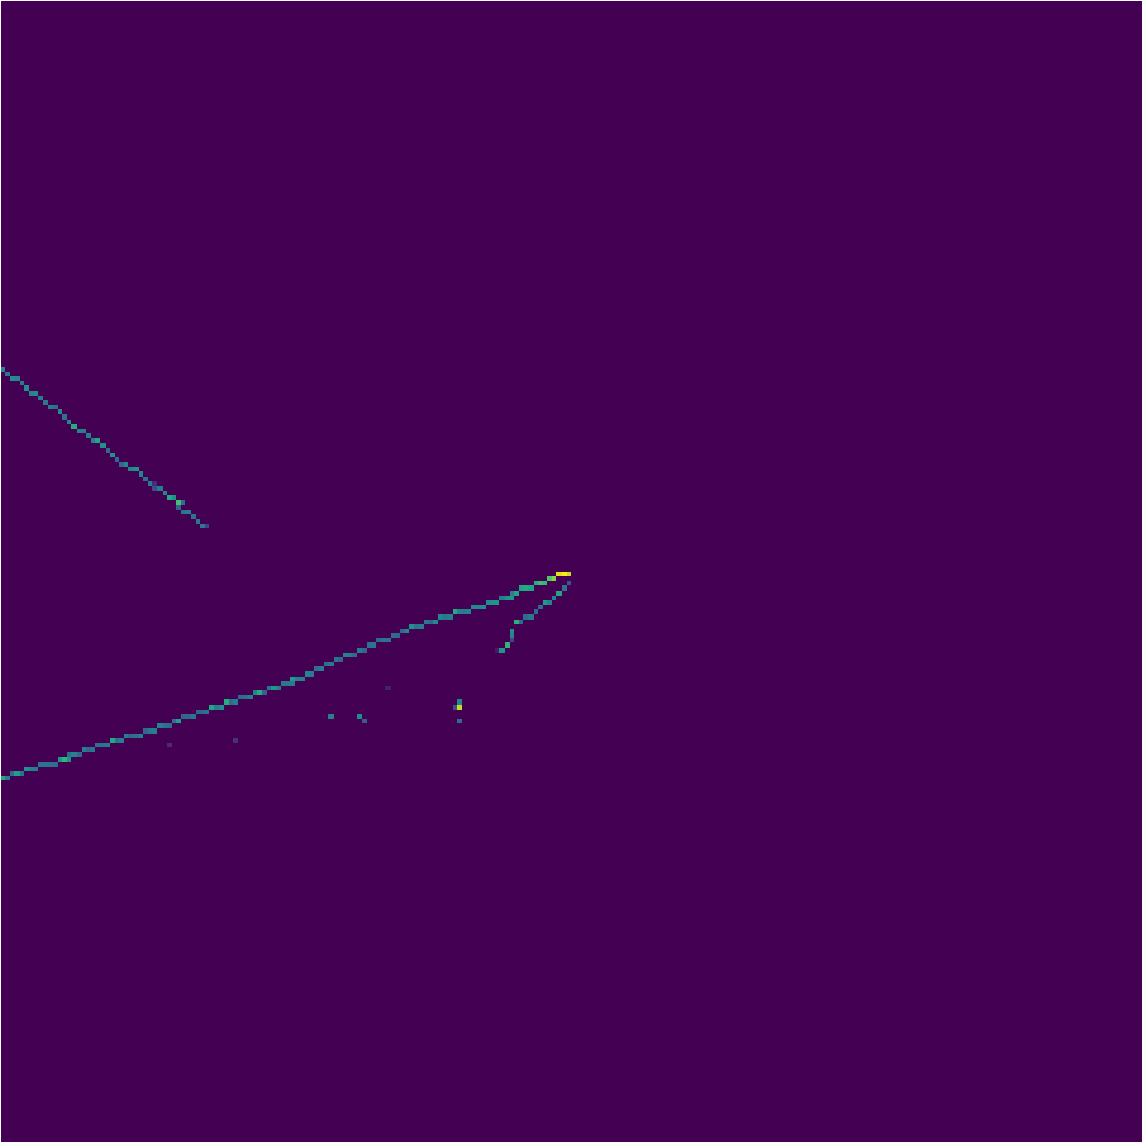
\includegraphics[width=\textwidth]{figures/unet_example_in.pdf}
		\caption {Input.}
		\label{fig:unet_example_in}
	\end{subfigure}

	\begin{tabularx}{\textwidth}{cc}
		\begin{subfigure}[b]{0.49\textwidth}
			\centering
			\vspace{3mm}
			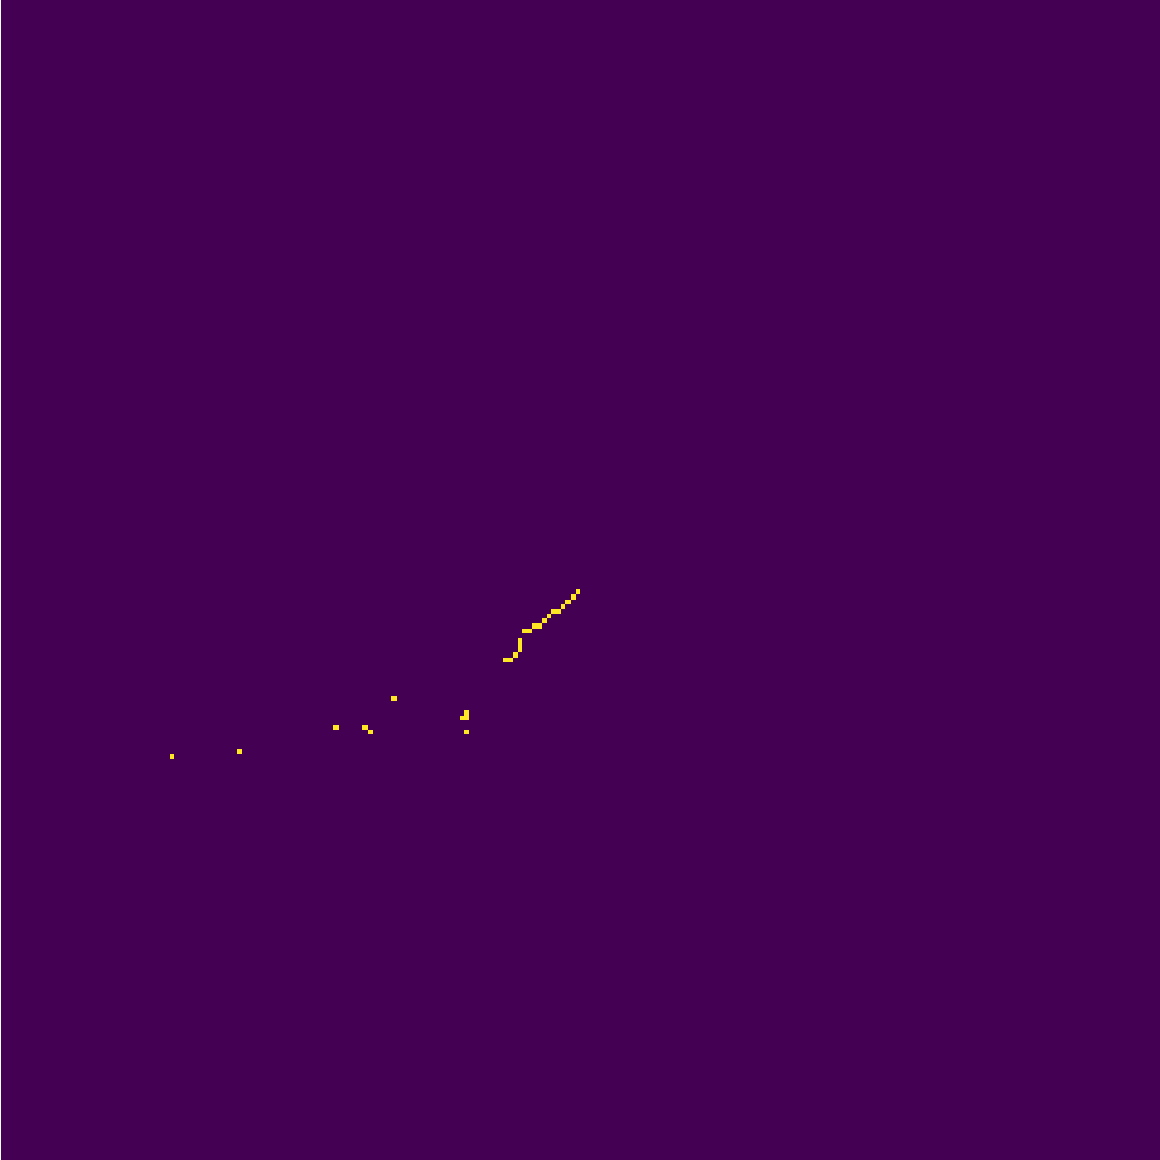
\includegraphics[width=\textwidth]{figures/unet_example_true.pdf}
			\caption {Truth.}
			\label{fig:unet_example_true}
		\end{subfigure} & 
		\begin{subfigure}[b]{0.49\textwidth}
			\centering
			\vspace{3mm}
			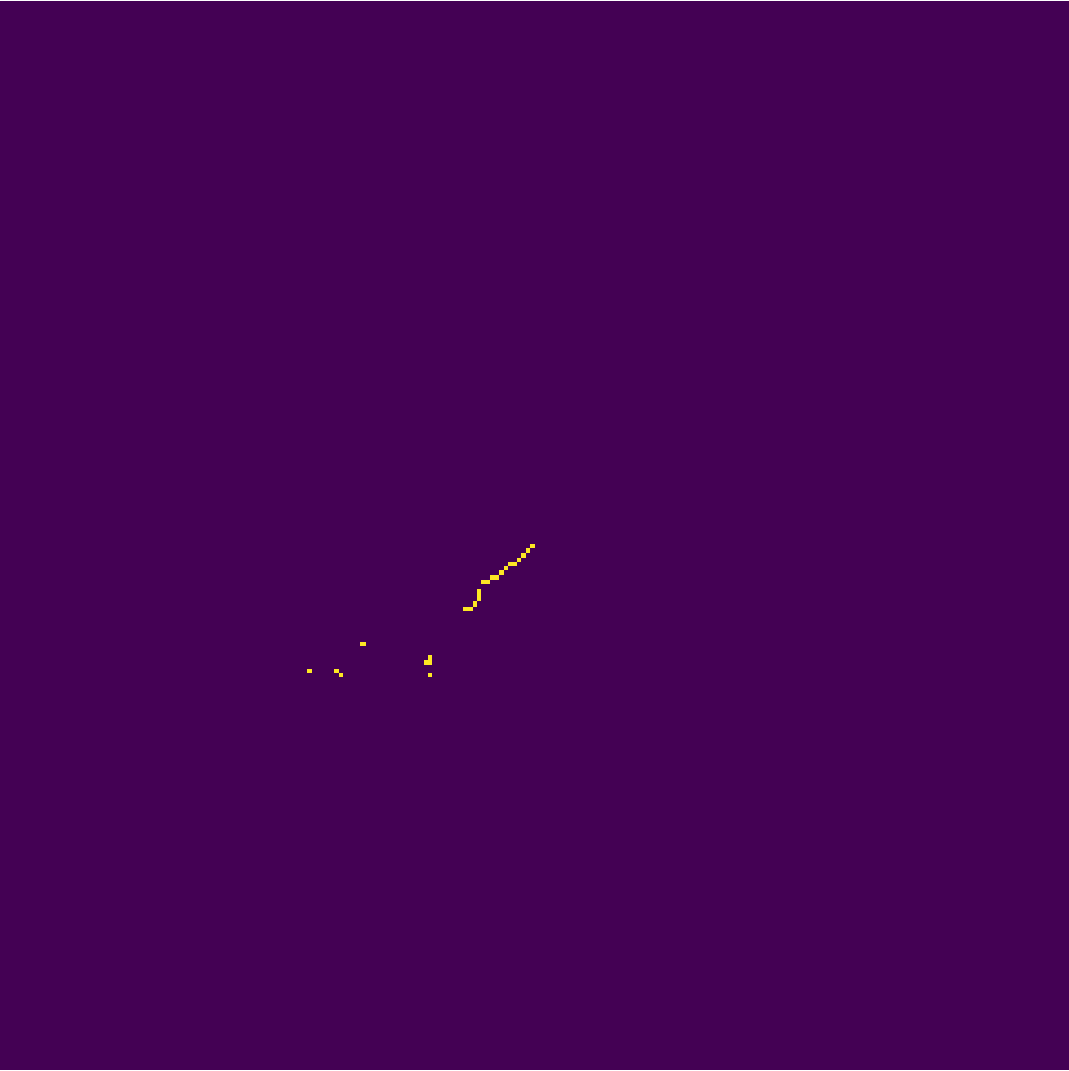
\includegraphics[width=\textwidth]{figures/unet_example_pred.pdf}
			\caption {Prediction.}
			\label{fig:unet_example_pred}
		\end{subfigure}
	\end{tabularx}

	\caption
	[Example input, true output, and prediction images for U-Net.]
	{Example input, truth, and prediction images for U-Net.}
	\label{fig:unet_example}
\end{figure}

\subsection{Michel Electron Reconstruction}

Michel electron reconstruction was evaluated on a dataset which was part of the 
same batch of simulation as the training, test, and validation data, but
distinct from all of them. 

\subsubsection{Hit Selection}

The U-Net produces a sharply peaked output distribution in both data and
simulation as seen in Figure \ref{fig:unet_pred_data}, the histograms here are
normalised by the number of entries. Both distributions show sharp peaks at zero
and one, but the distribution has slightly sharper peaks in simulation, which 
can be seen because the data has a tendency to be above the simulation for
scores far from zero and one. Hits from the input images are selected as 
Michel electron hits if their score exceed a selection threshold of 0.9. In 
simulation 7.8\% of hits are selected, while in data the fraction selected is 
8.0\%, therefore, there is a 2.5\% difference in the selected fraction between 
data and simulation.  
\begin{figure}
	\centering
	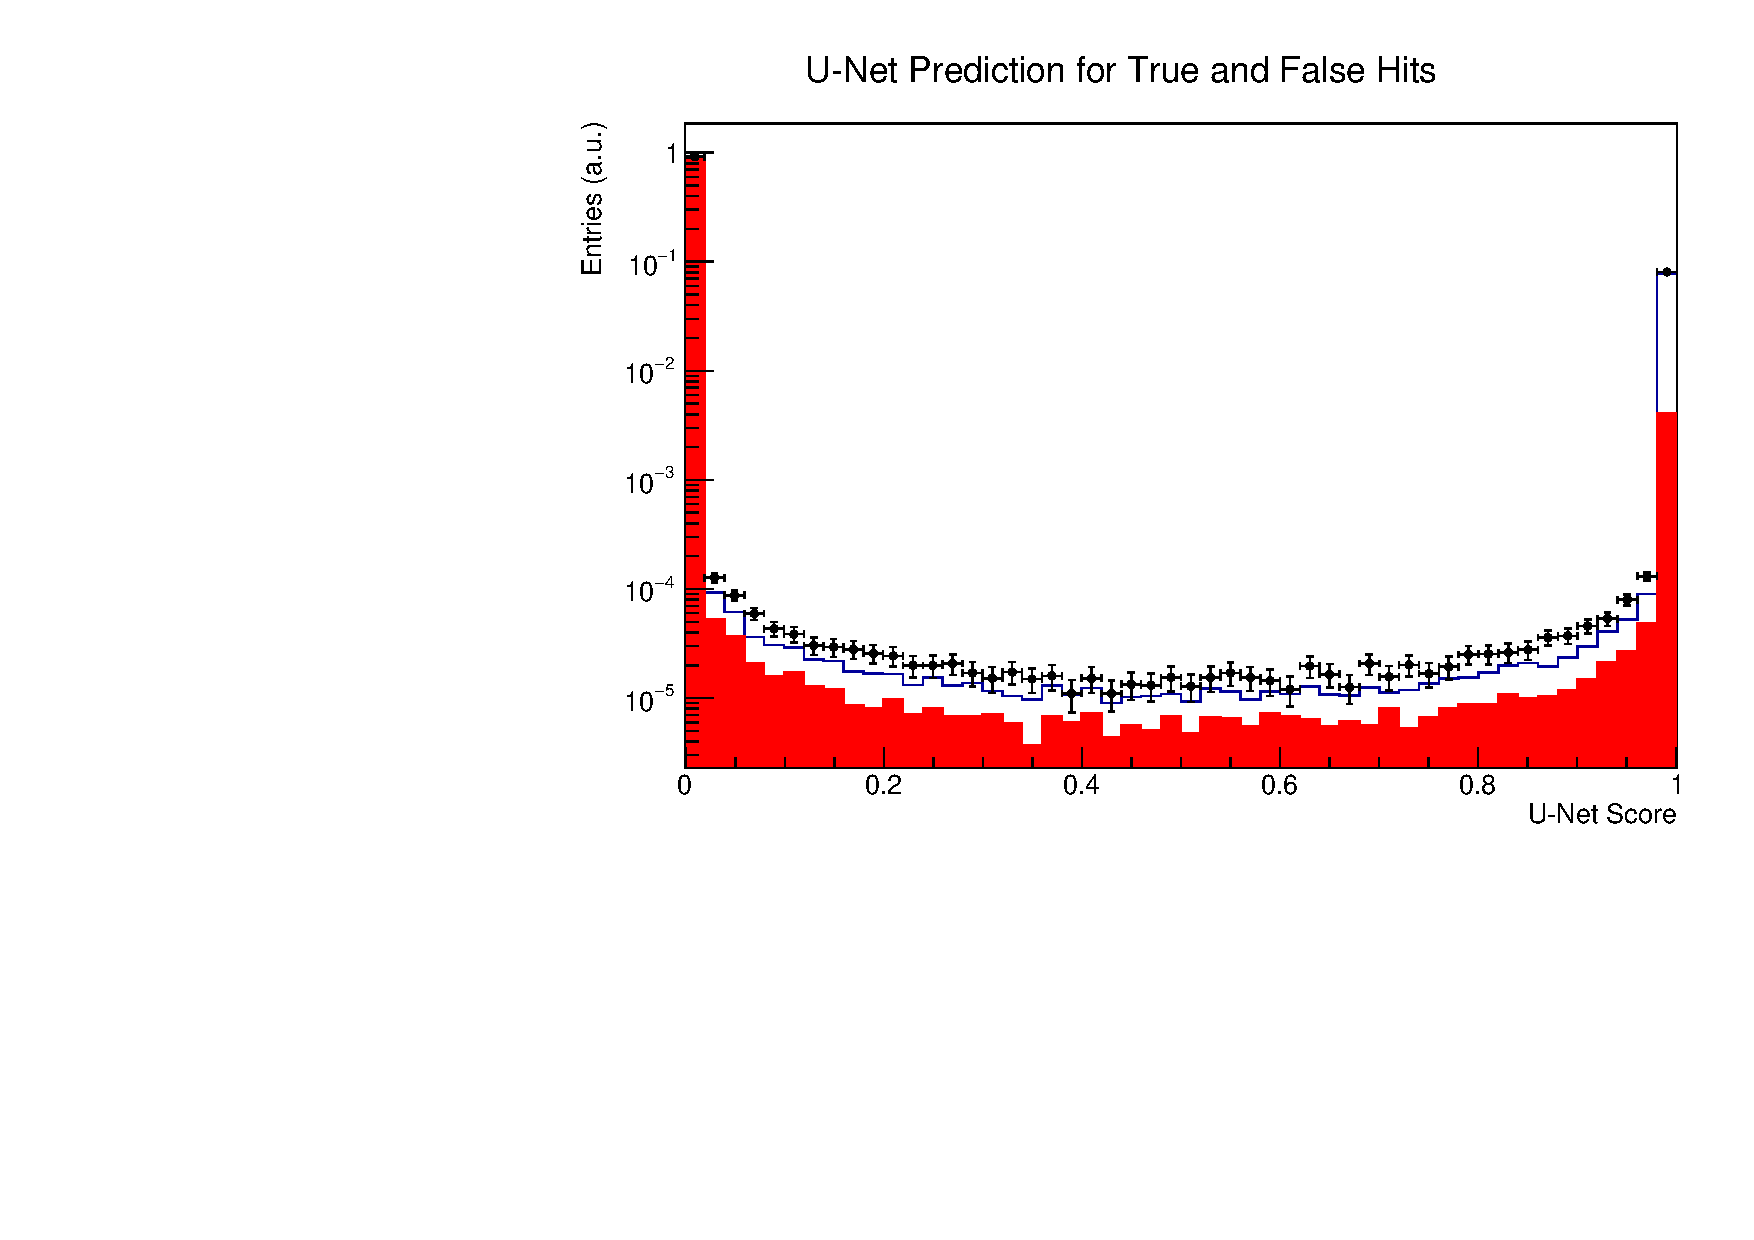
\includegraphics[width=\textwidth]{figures/unet_pred_data.pdf}
	\caption
	[U-Net Predicted Distribution.]
	{U--Net predicted distribution for hits in images. The simulated results are
	shown by the red line, with the backgrounds as a shaded red region. The data 
	is shown in black, with statistical error bars.}
	\label{fig:unet_pred_data}
\end{figure}

The performance of the hit tagging algorithm was analysed with the simulated
sample. Based on the score distributions for true and false hits the precision 
and completeness of the hit tagging algorithm can be evaluated. The precision 
and completeness are defined as 
\begin{align}
	\mbox{Precision} \quad &= \quad  \frac{N_{TP}}{N_{TP} + N_{FP}} \\
	\vspace{2mm}
	\mbox{Completeness} \quad &= \quad \frac{N_{TP}}{N_{TP} + N_{FN}}
\end{align}
where $N_{TP}$, $N_{FP}$, and $N_{FN}$ are the number of true--positives,
false--positives, and false--negatives respectively. These parameters give a
quantitative evaluation of the performance of the hit tagging algorithm,
allowing for comparison between different algorithms. 

The purity and completeness of the hit tagging was calculated for a range of 
selection thresholds in the range $[10^{-7}, 1 - 10^{-7}]$, Figure 
\ref{fig:unet_pur_comp} shows the purity against completeness for the values 
in this range. The hit tagging algorithm produces a high precision and 
completeness throughout the range of thresholds, however the steepness of the 
score distributions means that the choice of threshold makes little difference 
to the performance, meaning that little can be done to optimise the performance
by varying the threshold.
\begin{figure}
	\centering
	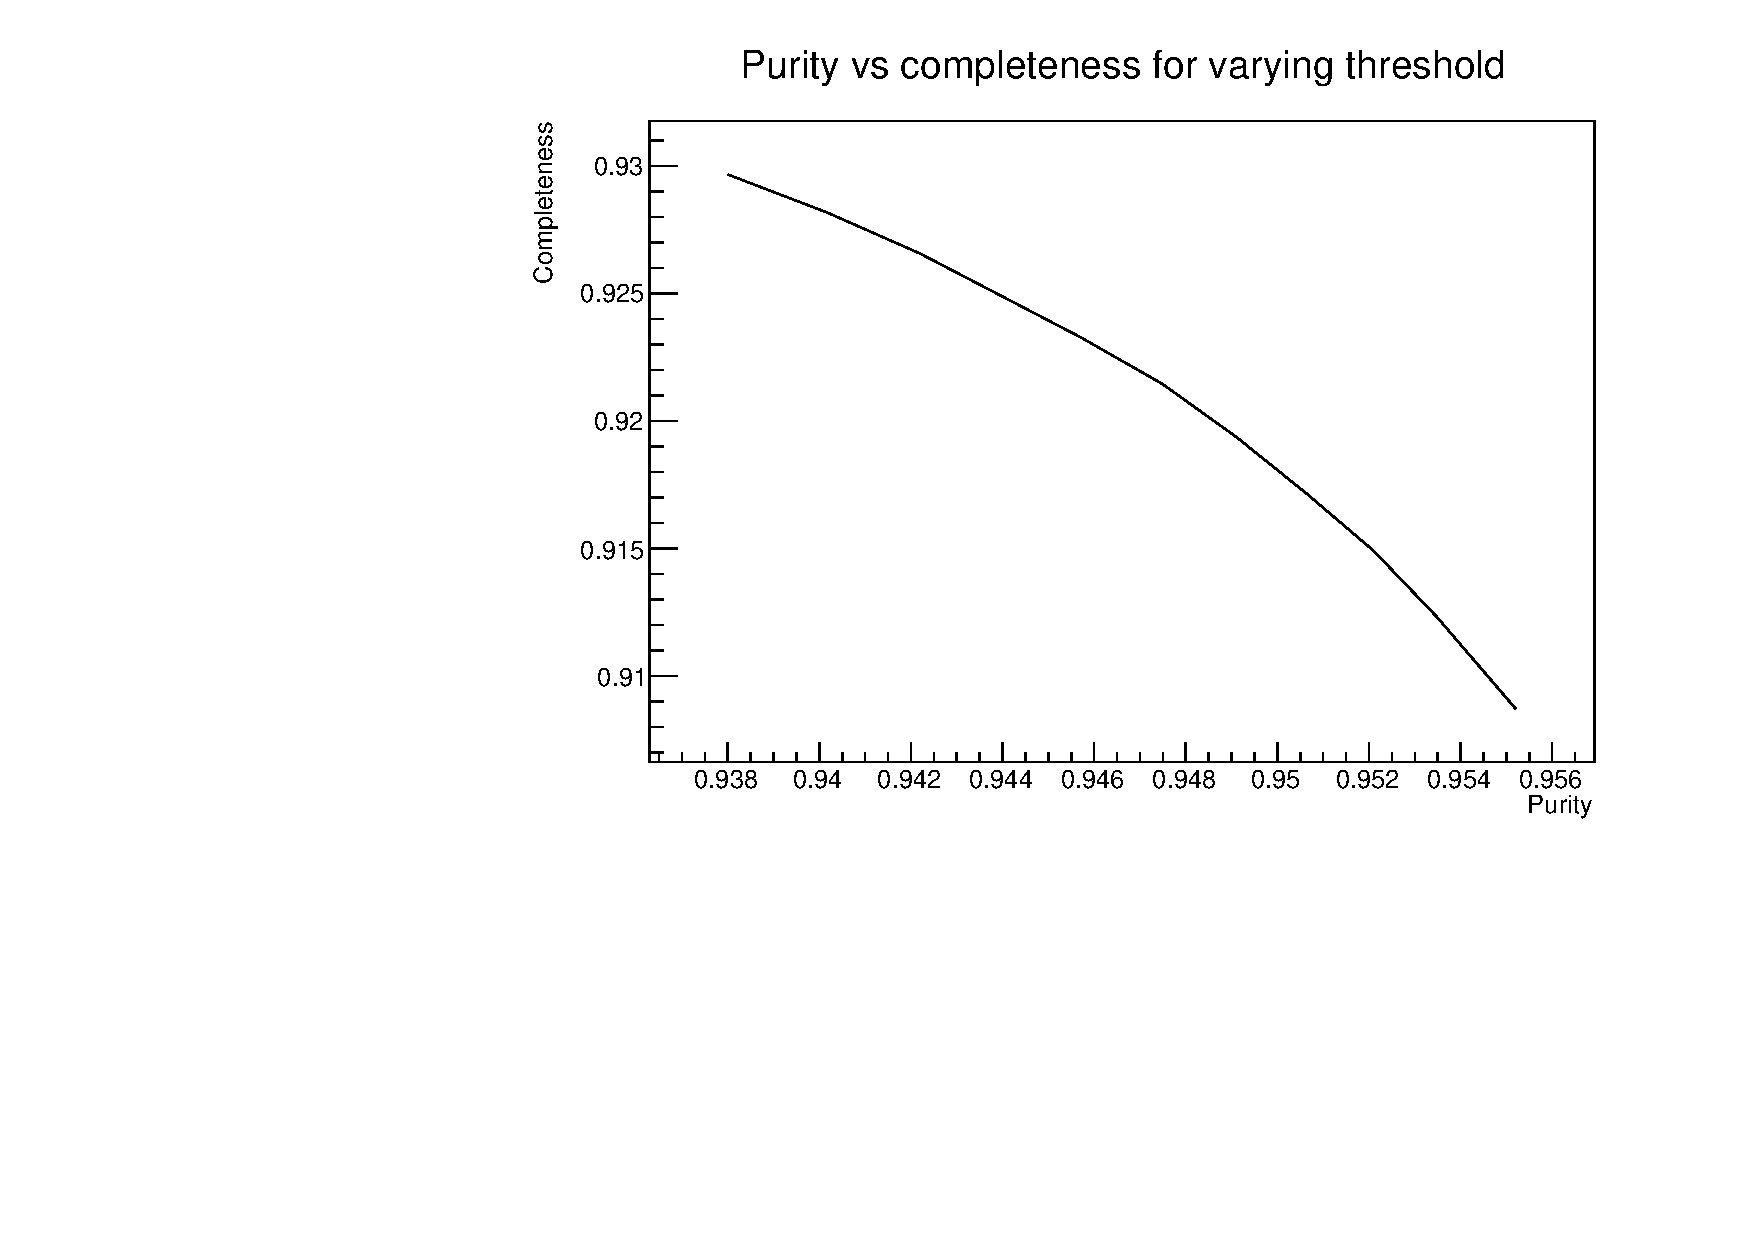
\includegraphics[width=\textwidth]{figures/unet_pur_v_comp.pdf}
	\caption
	[U-Net purity vs completeness.]
	{Hit tagging purity vs completeness for the U--Net algorithm on \protodune{}
	simulation.}
	\label{fig:unet_pur_comp}
\end{figure}

The number of hits selected per event for data and simulation is shown in 
figure \ref{fig:mich_n_hits}. Around 10 hits are selected on average per 
event, with a tail extending up to around 30 hits. The distribution of the
backgrounds follows a similar distribution to the true events. A good agreement
is seen between the data and simulation for the number of selected hits, these
hits are then used to reconstruct the deposited ionisation energy of the Michel
electron.
\begin{figure}
	\centering
	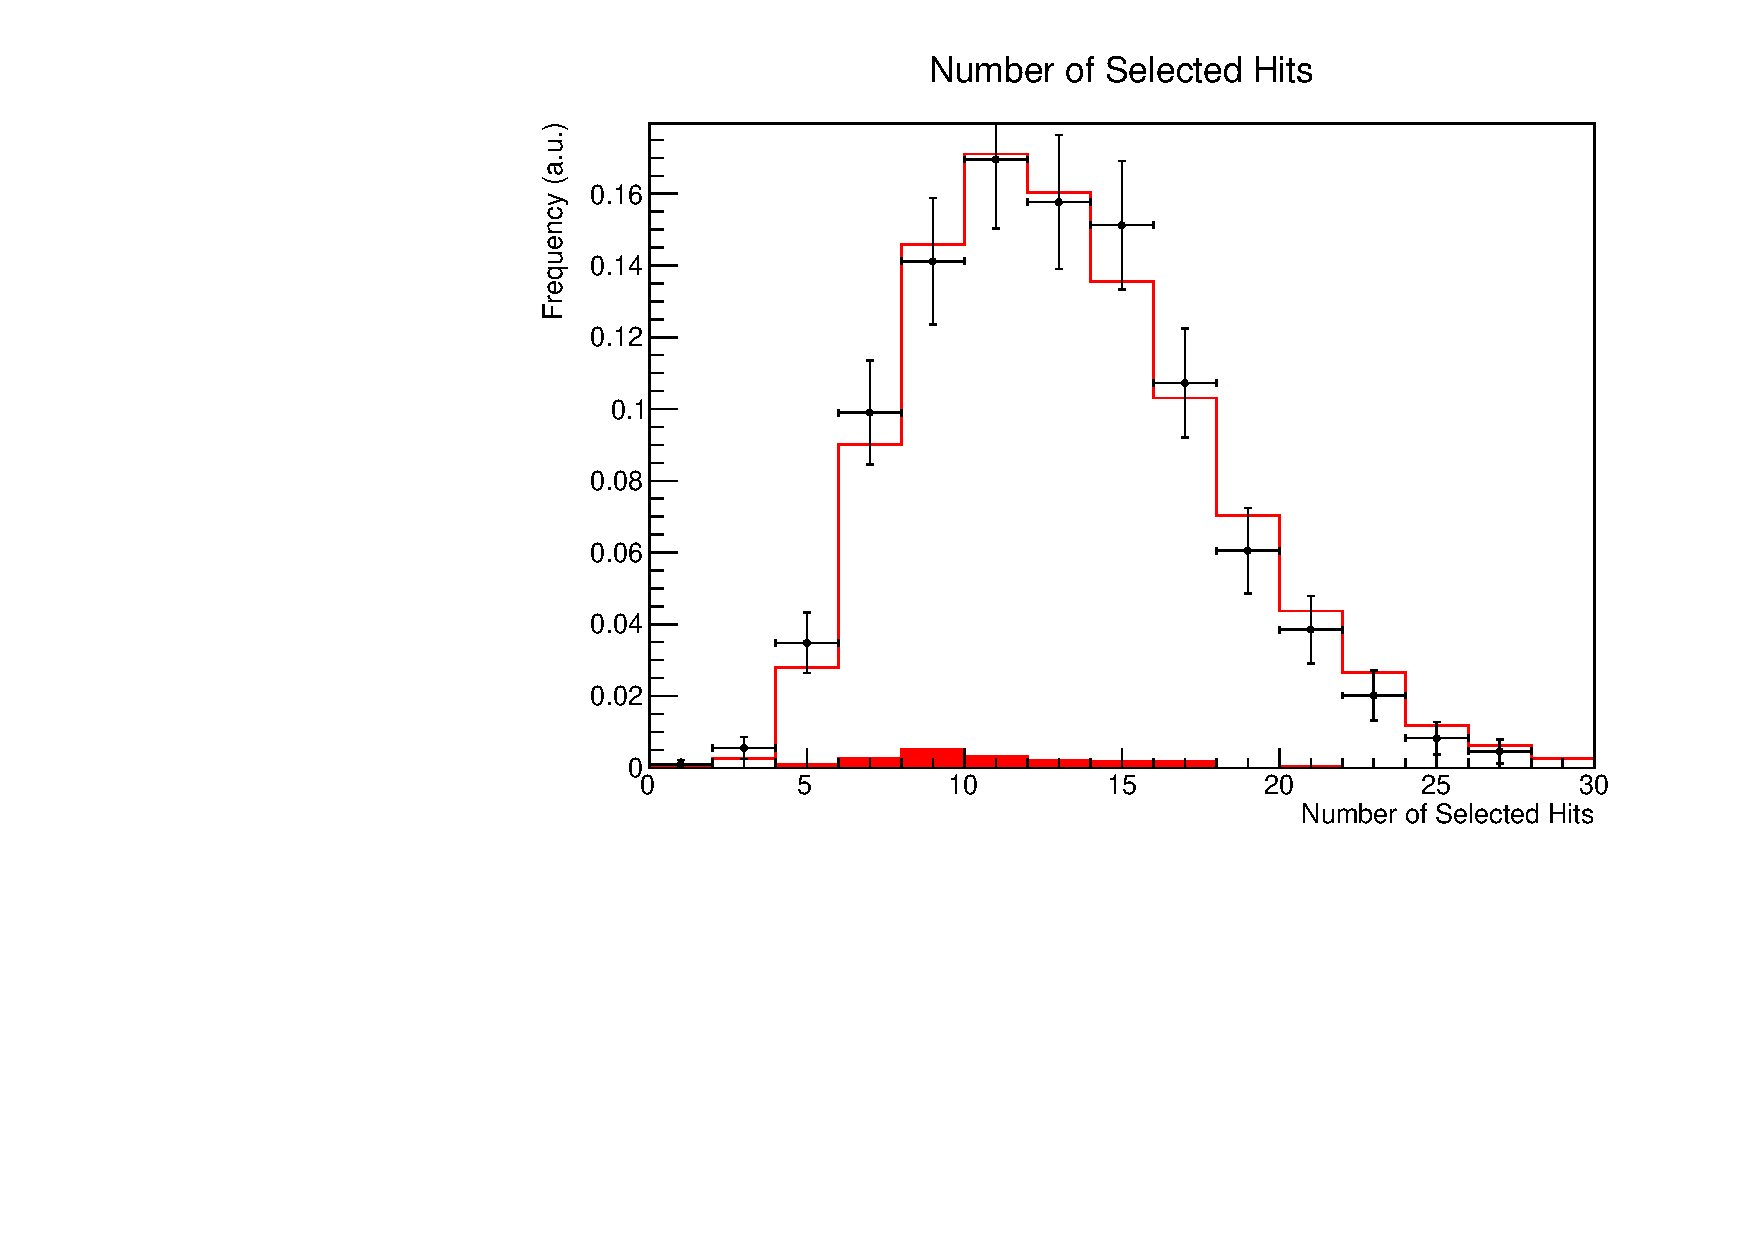
\includegraphics[width=\textwidth]{figures/mich_n_hits.pdf}
	\caption
	[Number of hits in Michel electron events.]
	{Number of hits selected by the U--Net for Michel electron candidate events in
	data and simulation.}
	\label{fig:mich_n_hits}
\end{figure}

\subsubsection{Ionisation Energy Reconstruction}

The total ionisation energy is reconstructed by summing the hit--by--hit
ionisation energy for all hits selected by the U-Net. The ionisation energy for
each hit is reconstructed from the hit integral in ADC as 
\begin{equation}
	E_{hit} = \frac{I_{hit} \times C_X \times C_{YZ} \times N \times W_{ion}}{C \times R}\mbox{,}
\end{equation}
where $E_{hit}$ is the reconstructed hit energy in MeV, $I_{hit}$ is the
integrated hit charge in ADC, $C_X$ is the X--correction factor which is
dependent on the X coordinate of the hit within the TPC, $C_{YZ}$ is the 
YZ--correction factor which is dependent on the Y and Z coordinates 
of the hit within the TPC, $N$ is a dimensionless normalisation factor which
normalises the data and MC distributions to give the same magnitude, $W_{ion}$
is the ionisation energy of argon in MeV per electron, $C$ is a constant
conversion factor which has units ADC per electron, and $R$ is the
recombination factor. The distribution of reconstructed hit energies in
\protodune{} data and simulation is shown in Figure \ref{fig:hit_ion_reco}.

The position dependent calibration matrices correct for non-uniformity in the
detector response across the TPC. In the X direction, which is parallel to the
drift direction, the main contributing factors are attenuation due to electron 
absorption, and variations in the electron drift velocity due to space charge 
effects. The main contributing factor for the YZ--correction factor are 
wire--to--wire response variations. 

As discussed in chapter \ref{ch:energyloss}, the recombination factor is a
$dE/dx$ dependent factor, which depends on the conditions in the liquid
argon. Due to the shortness of Michel electron tracks and the other charge 
deposits, it is challenging to assign $dE/dx$ on a hit--by--hit basis for this 
sample. Therefore, an average recombination factor is used for all hits. The 
recombination factor was calculated using the box model \cite{Acciarri2013a} 
under \protodune{} operating conditions, which gives an average value of 0.69.

As a result of the spatially dependent calibration factors, the energy of hits 
can only be accurately reconstructed for events with a reconstructed true 
time. This leads to a significant drop in event selection efficiency, which is 
due to the fact that only 15\% of cosmic--ray tracks have a reconstructed true 
time in simulation and only 1\% in data.

\begin{figure}
	\centering
	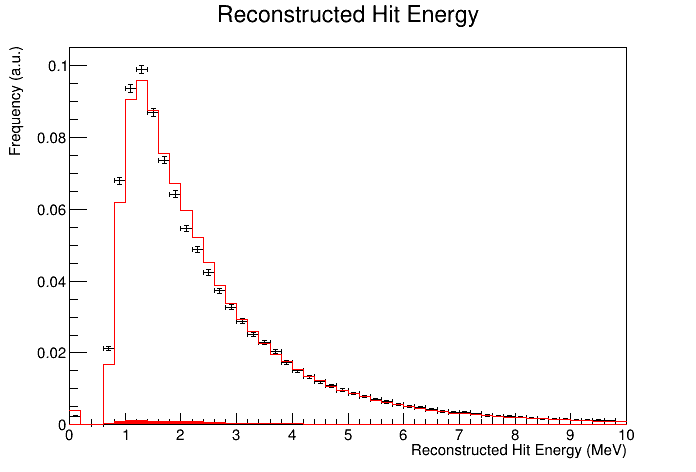
\includegraphics[width=\textwidth]{figures/hit_ion_reco.png}
	\caption
	[Reconstructed Hit Ionisation Energy.]
	{Reconstructed Hit Ionisation Energy for hits in Michel electron input images 
	in data and simulation.}
	\label{fig:hit_ion_reco}
\end{figure}

The reconstructed Michel electron energy is the sum of the reconstructed
ionisation energy for all selected Michel electron hits. The reconstructed 
ionisation energy spectrum for Michel electrons in \protodune{} is shown in 
Figure \ref{fig:michel_ion_reco}. The distribution peaks at around 20 MeV and 
has a tail up to just under 50 MeV, which is consistent with the true 
ionisation energy deposited by Michel electrons within a 40 cm radius, shown 
in Figure \ref{fig:40_v_80}.
\begin{figure}
	\centering
	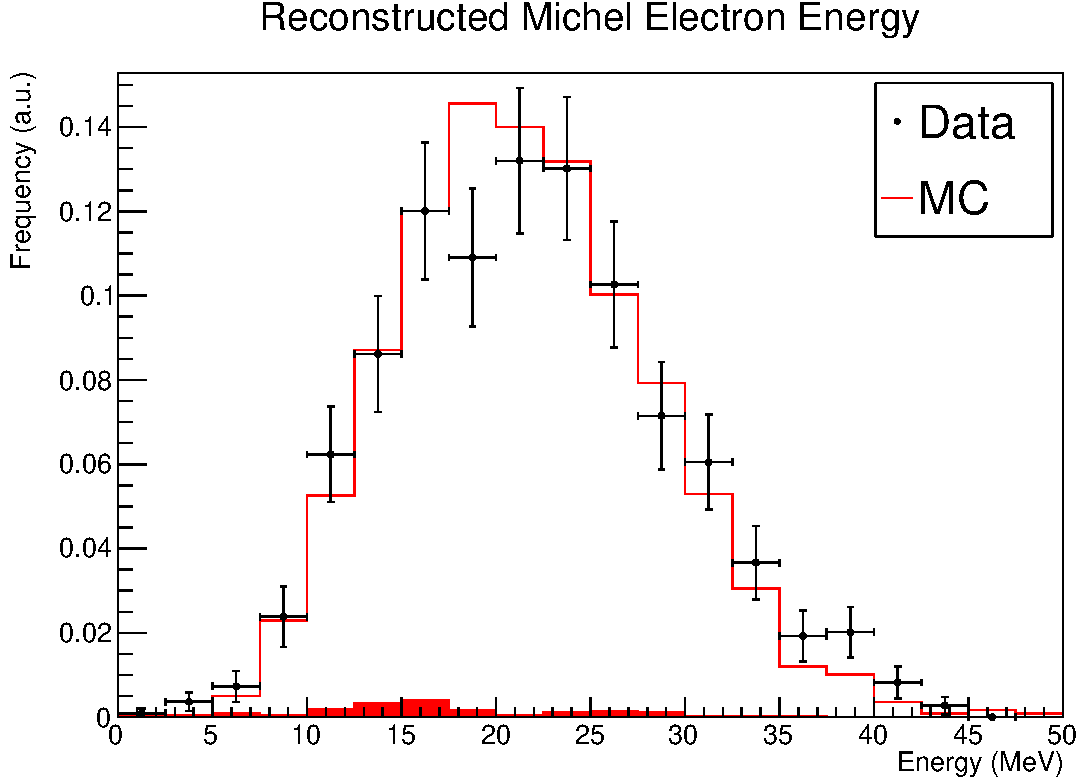
\includegraphics[width=\textwidth]{figures/michel_ion_reco.pdf}
	\caption
	[Reconstructed Michel Electron Ionisation Energy.]
	{Reconstructed Michel electron ionisation energy in data and simulation.}
	\label{fig:michel_ion_reco}
\end{figure}

The performance of the ionisation energy reconstruction was evaluated with the
simulated Michel electron sample. First, the reconstructed ionisation energy was
compared to the true ionisation energy, and a linear scaling factor was
calculated to correct for any energy offset. The correction factor was
calculated based on a liner fit to the distribution of reconstructed energy
against true energy, which is shown in Figure \ref{fig:reco_v_ion}. The
reconstructed energy was corrected based on this linear fit, 
\begin{equation*}
	E_{corr} = \frac{E_{reco}  - 0.808 \mbox{ MeV}}{0.9567},
\end{equation*}
and the corrected energy was used to estimate the energy resolution and bias of
the Michel electron energy reconstruction.
\begin{figure}
	\centering
	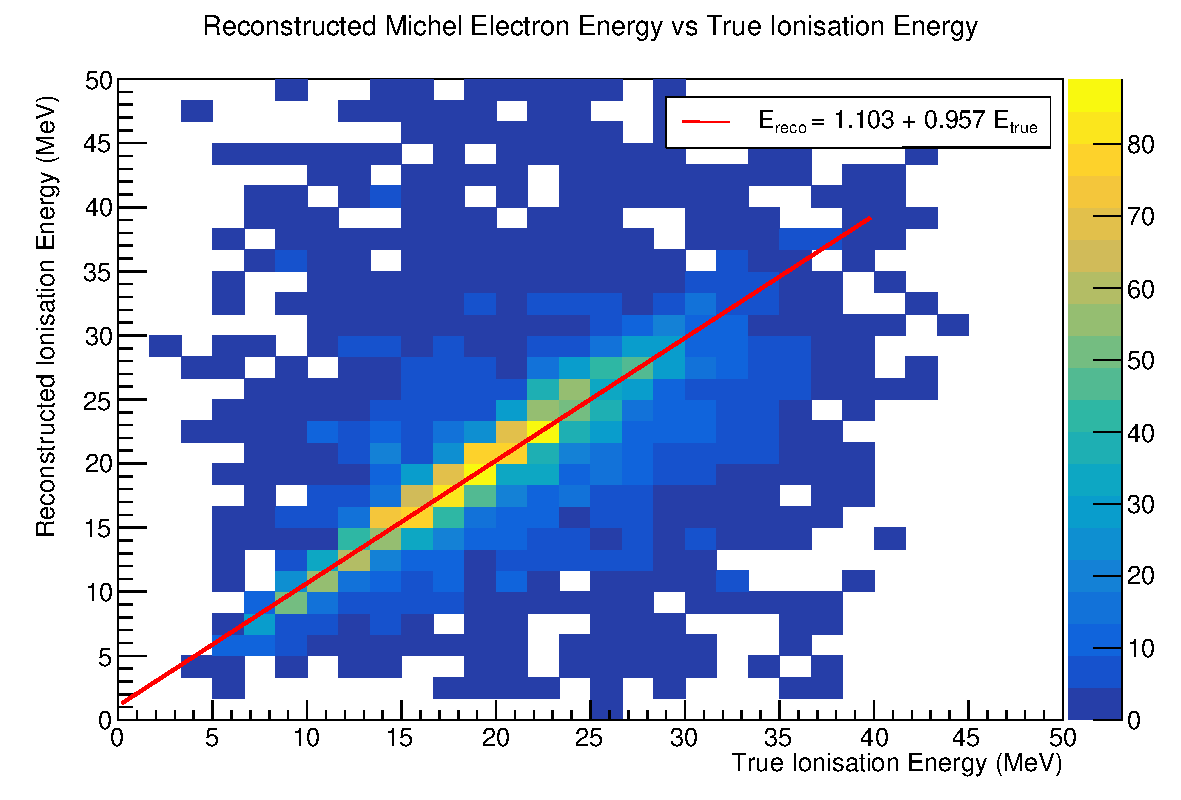
\includegraphics[width=\textwidth]{figures/reco_v_true_ion.pdf}
	\caption
	[Reconstructed Ionisation vs True Ionisation.]
	{Reconstructed Ionisation vs True Ionisation.}
	\label{fig:reco_v_ion}
\end{figure}

To estimate the resolution and bias of the ionisation energy reconstruction, the
fractional difference between the reconstructed and true ionisation energy was
considered. We define the fractional difference as,
\begin{equation*}
	\mbox{Fractional Difference} = \frac{E_{corr} - E_{true}}{E_{true}},
\end{equation*}
such that the spread of the distribution is a measure of the fractional
uncertainty of the reconstructed energy. The energy resolution and bias were
estimate by fitting a gaussian to the fractional difference distribution; the
standard deviation of the gaussian was taken to be an estimate of the energy
resolution, and the mean of the gaussian was taken to be an estimate of the
bias. The distribution of the fractional difference for all events, and the 
associated gaussian fit, are shown in Figure \ref{fig:frac_diff_ion}. Based on
this fit the energy resolution was estimated to be around 10\% and the bias 
around 1\%. However, it is worth noting that the fractional difference
distribution has a fairly significant tail for negative fractional differences,
and therefore the fit was restricted to the central region of the distribution.
\begin{figure}
	\centering
	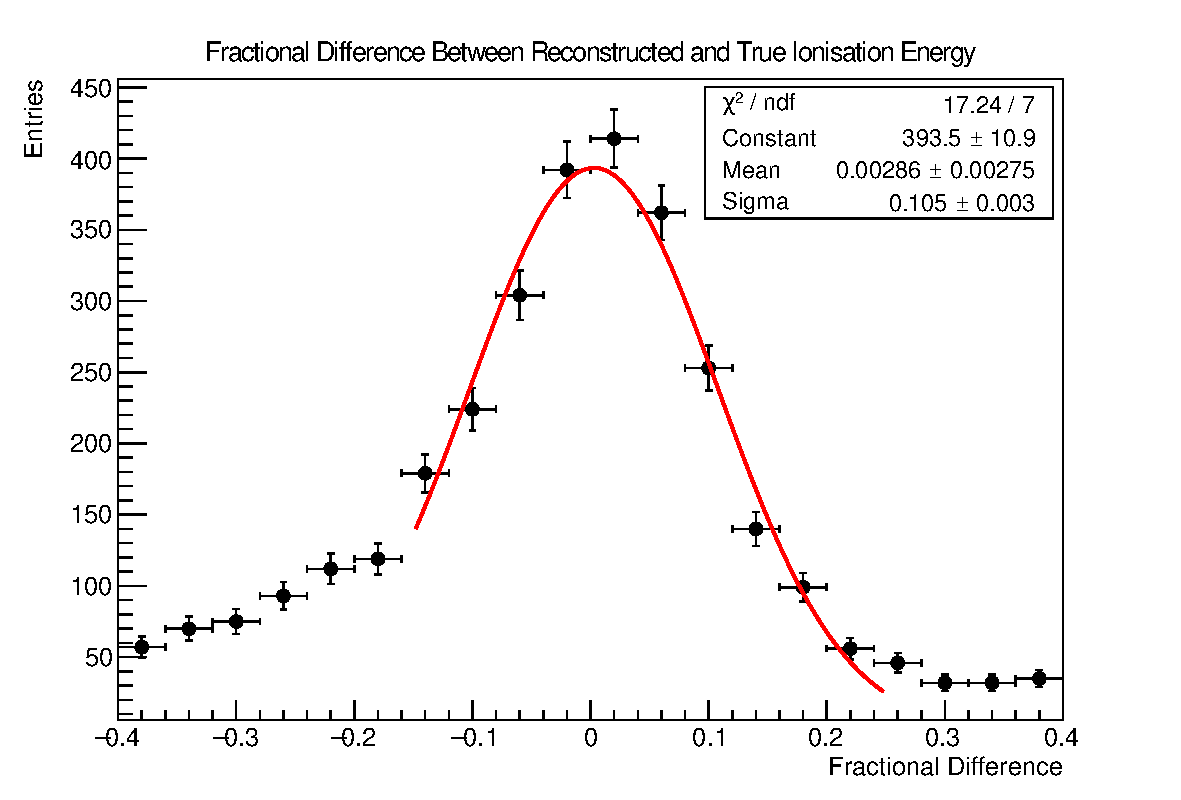
\includegraphics[width=\textwidth]{figures/frac_diff_ion.pdf}
	\caption
	[Fractional energy difference between reconstructed and true Michel electron
	energy.]
	{Fractional energy difference between reconstructed and true Michel electron
	energy.}
	\label{fig:frac_diff_ion}
\end{figure}

Studies into the energy resolution and bias as a function of energy gave
insights into the source of the tail in Figure \ref{fig:frac_diff_ion}. These
were investigated by binning the fractional energy difference distribution in
terms of true ionisation energy, and performing the same gaussian fit to the
fractional difference distribution for each energy bin, to estimate the energy
resolution and bias. The measured energy resolution and bias as a function of 
true ionisation energy are shown in Figure \ref{fig:res_and_bias_ion}, the 
associated fits are given in Appendix \ref{ch:energyfits}.
\begin{figure}
	\centering
	\begin{subfigure}[b]{\textwidth}
		\centering
		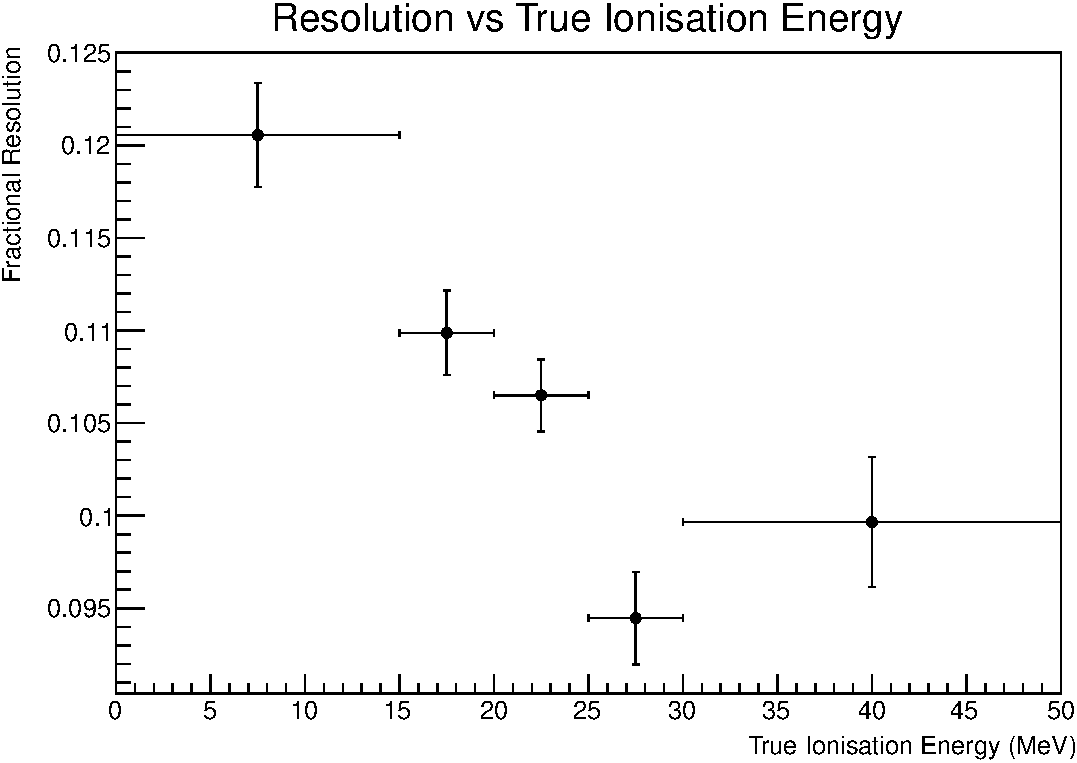
\includegraphics[width=0.95\textwidth]{figures/res_v_energy_ion.pdf}
		\caption {Resolution.}
		\label{fig:res_ion}
	\end{subfigure}
	\begin{subfigure}[b]{\textwidth}
		\centering
		\vspace{5mm}
		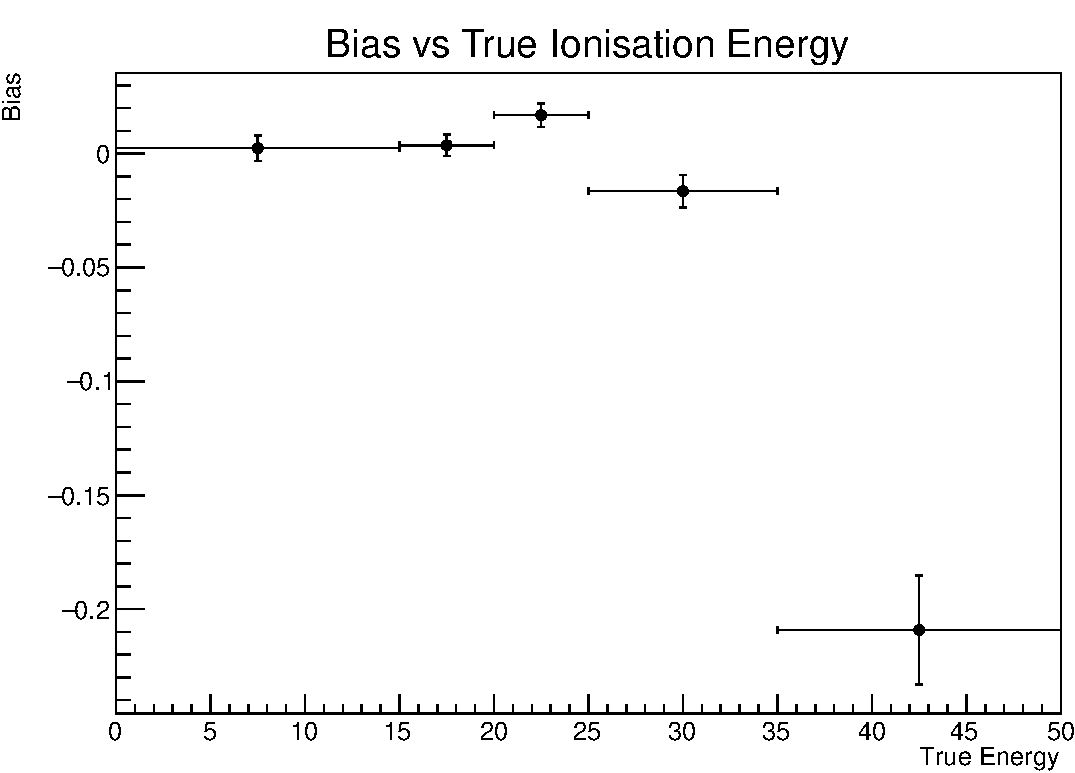
\includegraphics[width=0.95\textwidth]{figures/bias_v_energy_ion.pdf}
		\caption {Bias.}
		\label{fig:bias_ion}
	\end{subfigure}
	\caption
	[Energy resolution and bias as a function of true ionisation energy deposition.]
	{Energy resolution and bias as a function of true ionisation energy deposition.}
	\label{fig:res_and_bias_ion}
\end{figure}

% FIXME: you were here.
The energy resolution and bias as a function of energy demonstrates that the
energy reconstruction algorithm is capable of good energy reconstruction
performance. However, it is important to note that above around 25 MeV there is
significant tail for negative fractional differences. This is due to a reduction
in the hit tagging efficiency in the high energy region, which causes less of
the initial Michel electron energy to be collected by the CNN. No attempt was
made to fit this tail, and therefore the estimated energy resolution and bias
based on the gaussian fits, used to populate Figure \ref{fig:res_and_bias_ion},
overstate the performance in the high energy region. A more conservative 
estimate can be made by considering the mean and RMS of the distribution. 
Table \ref{tab:gaus_v_mean} gives a comparison between the estimated bias and 
resolution based on these two methods.
\begin{table}
	\centering
	\bgroup
	\def\arraystretch{1.5}
	\begin{tabular}{c|c|c|c|c}
		Energy Bin & Gaussian Mean & Gaussian Sigma & Mean    & RMS    \\ \hline
		0--15 MeV  & 0.0033        & 0.1206         & 0.0082  & 0.1501 \\
		15--20 MeV & 0.0175        & 0.1099         & 0.0176  & 0.1472 \\
		20--25 MeV & 0.0093        & 0.1065         & 0.0003  & 0.1452 \\
		25--30 MeV & -0.0010       & 0.0945         & -0.0338 & 0.1485 \\
		30--50 MeV & -0.02943      & 0.0997         & -0.0859 & 0.1603 \\
	\end{tabular}
	\egroup
	\caption
	[Comparison of energy resolution estimates for Michel electron ionisation
	energy.]
	{ Comparison of energy resolution estimates for Michel electron ionisation
	energy. }
	\label{tab:gaus_v_mean}
\end{table}

\subsubsection*{Contributions to Ionisation Energy Resolution}
The ionisation energy resolution is made up of a combination of the hit--by--hit
energy resolution, and the spread introduced due to imperfect hit tagging. The
contribution from the hit--by--hit energy resolution can be estimated by
considering the fractional energy difference in the case of perfect hit tagging,
which sums up the reconstructed energy of all the true Michel electron hits in
the image. The sum over the hits in each image is considered because this
allows the error in the hit--by--hit recombination factor, which arises due to
the use of an average recombination factor during reconstruction, to be 
averaged over the hits in the image. The fractional energy difference in this
case is fit with a gaussian distribution, which is shown in Figure
\ref{fig:michel_hit_res}. 
\begin{figure}
	\centering
	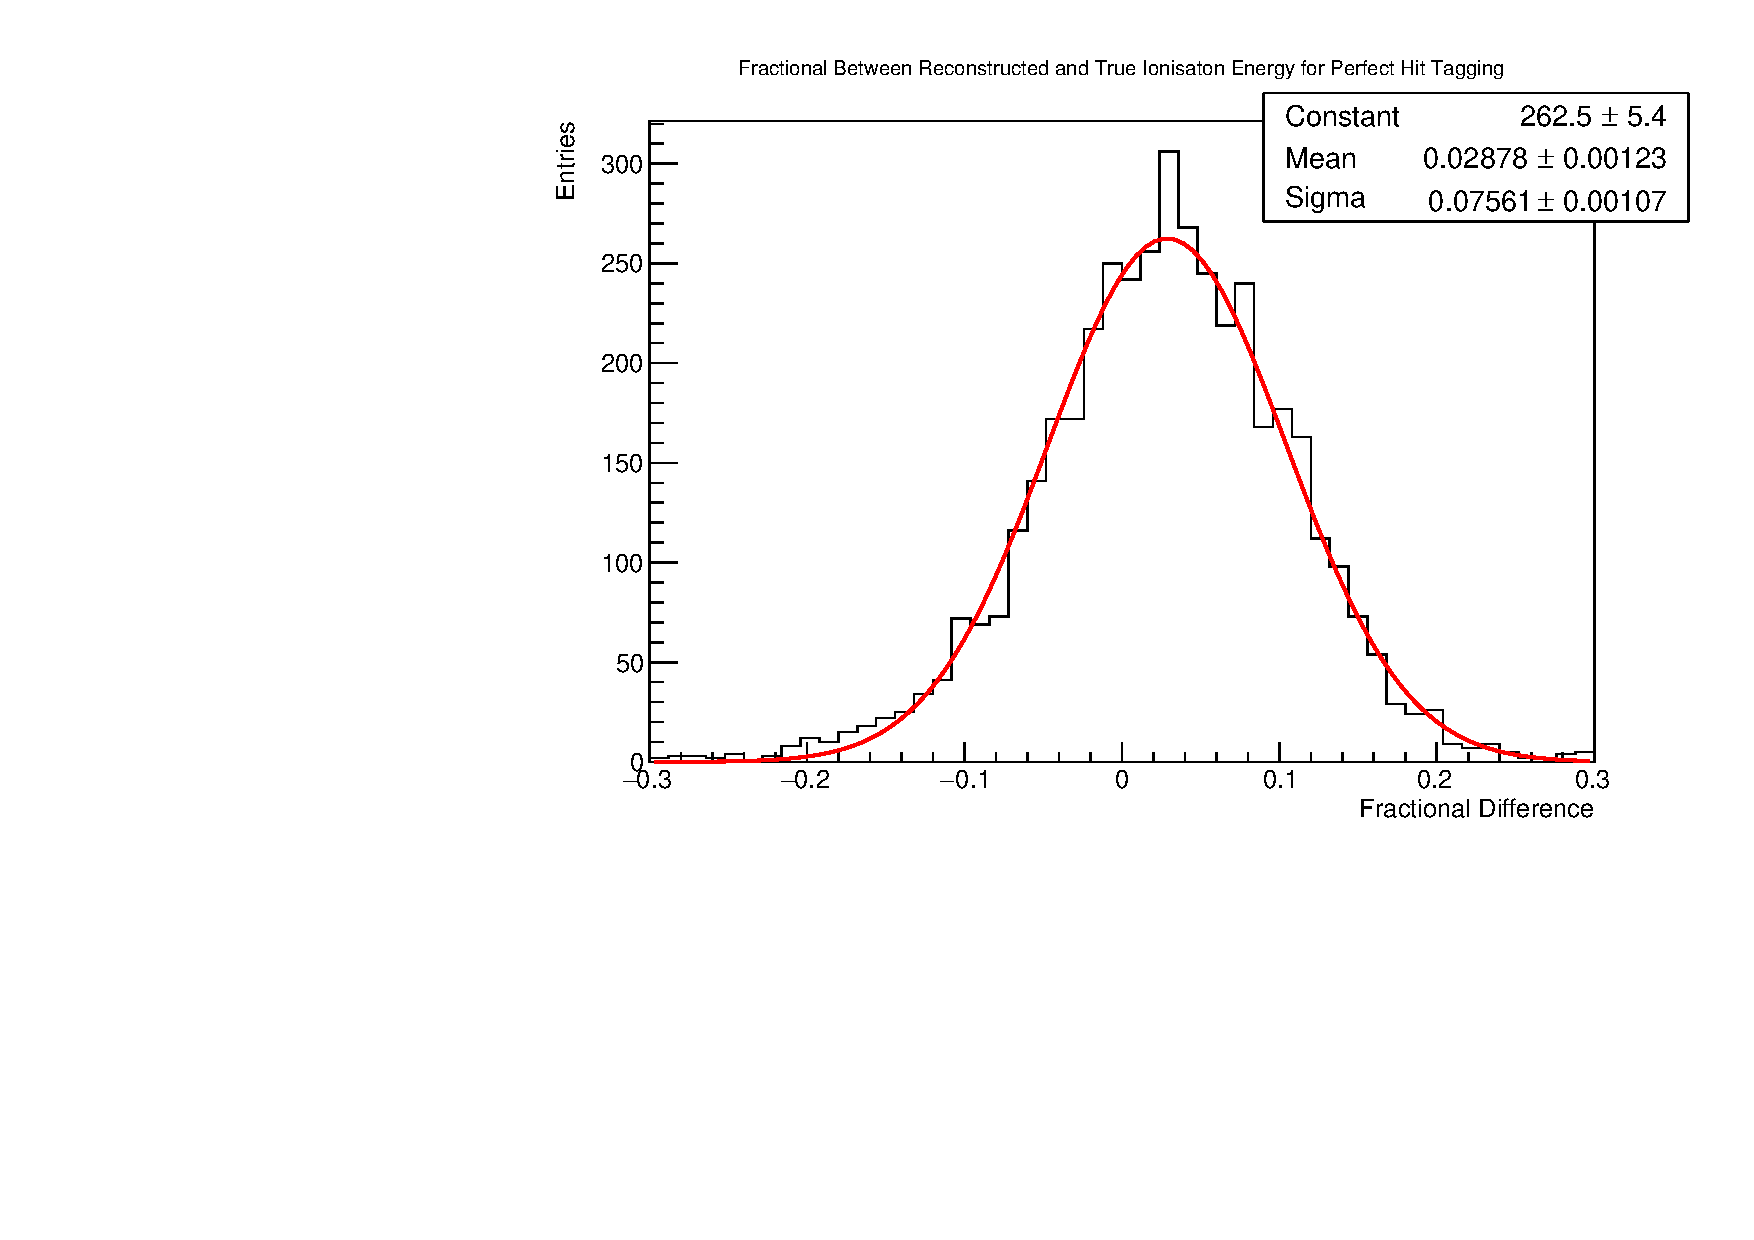
\includegraphics[width=\textwidth]{figures/michel_hit_energy_resolution.pdf}
	\caption
	[Energy uncertainty contribution from hit energy reconstruction.]
	{The fractional difference between the true ionisation energy deposition and
	the reconstructed ionisation energy deposition for Michel electron
	reconstructed with perfect hit tagging. The distribution is fit with a 
	gaussian, which is shown in red, and the fit parameters are shown in the top 
	right corner. The error bars are statistical.}
	\label{fig:michel_hit_res}
\end{figure}

The contribution to the ionisation energy resolution due to the hit energy
reconstruction was estimated based on the parameters from the gaussian fit in
Figure \ref{fig:michel_hit_res}. The bias in the hit energy reconstruction was 
estimated to be around 3\%, and the resolution was estimated to be 
approximately 8\%. The remaining energy resolution and bias seen in the Michel 
electron ionisation energy reconstruction is a result of the spread due to 
imperfect hit tagging.

\subsubsection*{Comparison to Other LArTPC Experiments} \label{ME_COMP}

In order to put the performance of the Michel electron energy
reconstruction into context, it is useful to compare the results presented 
here with those from other LArTPC experiments. We will restrict the 
comparisons here to the 0--30 MeV region for this comparison, recognising that 
improvements are still required in order to reduce the tail for higher energy 
ionisation energies.  The closest comparison is against the MicroBooNE 
experiment, which is a surface level LArTPC which used ionisation energy for 
the reconstruction\cite{Acciarri2017}. LArIAT and ICARUS have also performed 
Michel electron reconstruction\citetemp{Amoruso:2003sw,Foreman_2016}, however, 
LArIAT used the scintillation light for reconstruction, and ICARUS is deep 
underground and therefore has significantly less backgrounds.

The closest comparison for Michel electron energy reconstruction comes from the
MicroBooNE LArTPC; both MicroBooNE and \protodune{} are surface level TPCs, and
they both use ionisation energy for Michel electron reconstruction. In
MicroBooNE, the ionisation energy resolution for Michel electrons was found to
be between 15--25\% in the 0--30 MeV region\cite{Acciarri2017}. In this region
the algorithm developed here gives an improved energy resolution of around
10\%, which highlights the potential of the semantic segmentation approach if
the bias at higher energies can be improved.

ICARUS also used ionisation energy for Michel electron reconstruction, however,
the ICARUS detector was located deep underground, and therefore they were
subject to much lower backgrounds. In ICARUS the ionisation energy resolution 
was measured to be in the range of 3--8\%\cite{Amoruso:2003sw}, however, these
results did not take into account any radiated energy deposits, which form an
important part of the Michel electron signature. Therefore, the results from
ICARUS are not directly comparable to the measured energy resolution presented
here.

LArIAT is a significantly smaller TPC than \protodune{}, and therefore, despite
being at surface level, there is a sufficiently low rate of cosmic rays that the
photon detection system could be used to tag and measure Michel electron events.
LArIAT measured an energy resolution on the order of 20\% for Michel electrons 
based on the scintillation light signal\cite{Foreman_2016}. 

In DUNE, TODO.

\section{Conclusion} \label{ME_EU}

In the energy regime of Michel electrons, and supernova neutrinos, the
electromagnetic energy deposition of electrons moves from a ionisation dominated
to a radiation dominated region. As such, these events have a signature which
contains both track--like and a shower--like components, and therefore they 
require a unique reconstruction algorithm in order to maximise the energy 
collected from the events. 

In this chapter we have presented a novel Michel electron reconstruction
algorithm based on machine learning techniques. A sample of Michel electrons was
selected in \protodune{} data with a purity of over 98\% and an overall
efficiency of around 5\%. The ionisation energy of these events was
reconstructed based on a semantic segmentation algorithm, which uses a U--Net
CNN architecture. The performance of this algorithm shows an improvement in
energy resolution over similar experiments, with an ionisation energy resolution
of around 10-15\%. However, there is still need for improvement, particularly 
in the high energy region where a large tail is seen in the fractional 
difference distribution. 

% FIXME: you were here.
The promising results in the low energy region based on this method, suggest
that with further study the semantic segmentation approach could prove to be an
effective algorithm for reconstructing low energy particles in LArTPCs. However,
more work is required to ensure good performance across the desired energy
range. In order to increase the performance in the high energy region, we could 
consider increasing the amount of training data in the high energy region. At
the time of writing, there is currently insufficient \protodune{} simulation,
to produce a training sample which is flat across the full Michel electron energy range. Therefore,
this remains as a possible future study into improving the performance of this
algorithm.
